\documentclass{article}

\usepackage[math]{anttor}
\usepackage[T1]{fontenc}

\usepackage[all]{xy}

\usepackage{amsmath}
\usepackage{amssymb}
\usepackage{fullpage}
\usepackage{array}
\usepackage{MnSymbol,wasysym}

\usepackage{xcolor}
\definecolor{mylinkcolor}{rgb}{0.0,0.4,1.0}
\definecolor{mycitecolor}{rgb}{0.0,0.4,1.0}
\definecolor{shadecolor}{rgb}{0.89,0.88,0.80}

\usepackage[unicode,colorlinks=true,linkcolor=mylinkcolor,citecolor=mycitecolor]{hyperref}

\newcommand{\refref}[2]{\hyperref[#2]{#1 \ref*{#2}}}
\newcommand{\eqnref}[1]{\hyperref[#1]{(\ref*{#1})}}

\usepackage{amsthm}
\newtheorem{proposition}{Proposition}[section]
\newtheorem{lemma}[proposition]{Lemma}
\newtheorem{fact}[proposition]{Fact}
\newtheorem{conjecture}[proposition]{Conjecture}
\newtheorem{theorem}[proposition]{Theorem}
\newtheorem{corollary}[proposition]{Corollary}
\newtheorem*{claim}{Claim}
\theoremstyle{definition}
\newtheorem{example}[proposition]{Example}
\newtheorem{definition}[proposition]{Definition}
\newtheorem{observation}[proposition]{Observation}

\renewcommand{\Re}{\mathop{\mathrm{Re}}}
\renewcommand{\Im}{\mathop{\mathrm{Im}}}

\DeclareMathOperator{\Spec}{Spec}
\DeclareMathOperator{\supp}{supp}
\DeclareMathOperator{\rk}{rk}
\DeclareMathOperator{\Tr}{Tr}
\DeclareMathOperator{\End}{End}
\DeclareMathOperator{\rad}{rad}
\DeclareMathOperator{\fchar}{char}
\DeclareMathOperator{\Hom}{Hom}
\DeclareMathOperator{\Gal}{Gal}
\DeclareMathOperator{\GL}{GL}
\DeclareMathOperator{\ord}{ord}
\DeclareMathOperator{\Div}{Div}
\DeclareMathOperator{\DivC}{DivC}
\DeclareMathOperator{\Pic}{Pic}
\DeclareMathOperator{\Jac}{Jac}
\DeclareMathOperator{\Alb}{Alb}
\DeclareMathOperator{\disc}{disc}
\DeclareMathOperator{\Vol}{Vol}

\newcommand{\legendre}[2]{\left(\frac{#1}{#2}\right)}

\newcommand{\isom}{\simeq}
\newcommand{\term}{\textbf}
\newcommand{\dfn}{\mathrel{\mathop:}=}
\newcommand{\rdfn}{=\mathrel{\mathop:}}

\newcommand{\NN}{\mathbb{N}}
\newcommand{\ZZ}{\mathbb{Z}}
\newcommand{\FF}{\mathbb{F}}
\newcommand{\QQ}{\mathbb{Q}}
\newcommand{\CC}{\mathbb{C}}
\newcommand{\RR}{\mathbb{R}}
\newcommand{\PP}{\mathbb{P}}
\renewcommand{\AA}{\mathbb{A}}
\renewcommand{\O}{\mathcal{O}}

\renewcommand{\mod}{\mathop{\,\mathrm{mod}\,}}

\usepackage{framed}

\newenvironment{remark}
{ \begin{shaded}\begingroup\small\noindent\refstepcounter{proposition}\textbf{Remark \theproposition.} }
{ \endgroup\end{shaded} }

\usepackage{graphicx}

\newcolumntype{x}[1]{>{\centering\hspace{0pt}}p{#1}}

\newcommand{\seprule}{\rule{2cm}{1.5pt}}

\title{Heights}
\author{Lectures by Fabien Pazuki}
\date{Spring semester 2014}

\begin{document}
\maketitle

\noindent These are my notes from a course given by Fabien Pazuki at
Universit\'e de Bordeaux.
All typos and mistakes are mine, so please report them to
\texttt{cadadr@gmail.com}.
The last version of this text can be found at \url{https://cadadr.org/}

\iffalse
Currently there are three major omissions: in \refref{\S}{section:lehmer} the
Dobrowolski theorem is not proved (an exposition can be found in the book by
Bombieri and Gubler); in \refref{\S}{section:mordell} the Vojta's inequality is
assumed without any hint at its proof (a whole chapter of the book by Hindry and
Silverman is devoted to this); in \refref{\S}{section:faltings} the overview of
the Faltings' proof is far from being complete (it can be found in the notes of
J. Milne on abelian varieties).
\fi

\vspace{1em}

The recommended books:

\begin{itemize}
\item Marc Hindry, Joseph H. Silverman,
  \emph{Diophantine Geometry: An Introduction}

\item Enrico Bombieri, Walter Gubler, \emph{Heights in Diophantine Geometry}
\end{itemize}

\tableofcontents

\vspace{1em}

Heights is a fundamental tool in proving finiteness results in Diophantine
geometry and counting the resulting finite sets.

First we would like to define the height $H (\alpha)$ of an algebraic number
$\alpha \in \overline{\QQ}$, in a way that there are finitely many numbers
$\alpha$ with bounded height $H (\alpha) \le C$ and degree. For this one should
consider the absolute values of $\alpha$.

For example, the number $\frac{2014}{2013}$ is very close to $1$ with respect to
the usual absolute value $|\cdot|$. However, it carries a lot of arithmetic
information, since it contains primes $3\cdot 11\cdot 61 = 2013$ and
$2\cdot 19\cdot 53 = 2014$. So for instance its $2$-adic or $3$-adic absolute
value is far from $1$. The idea of a height is to put all the absolute values
together.

\section{Absolute values and product formula}

First we recall some definitions and facts about absolute values on fields.

\begin{definition}
  Let $K$ be a field. An \term{absolute value} on $K$ is a function
  $|\cdot|\colon K\to \mathbb{R}_{\ge 0}$ satisfying the following properties:

  \begin{enumerate}
  \item $|\alpha| = 0$ iff $\alpha = 0$.

  \item Multiplicativity: $|\alpha\,\beta| = |\alpha|\cdot |\beta|$ for all
    $\alpha,\beta\in K$.

  \item Triangle inequality: $|\alpha + \beta| \le |\alpha| + |\beta|$ for all
    $\alpha,\beta\in K$.
  \end{enumerate}

  If holds a stronger inequality
  $|\alpha + \beta| \le \max \{ |\alpha|, ~ |\beta| \}$, then the absolute value
  is called \term{nonarchimedian}.
\end{definition}

\begin{definition}
  Two absolute values $|\cdot|_1$ and $|\cdot|_2$ on $K$ are \term{equivalent}
  if there exists some number $\lambda > 0$ such that
  $|\cdot|_1 = |\cdot|_2^\lambda$.

  An equivalence class of absolute values on $K$ is called a \term{place}.
\end{definition}

\begin{theorem}[Ostrowski]
  On $\QQ$ any nontrivial absolute value is equivalent to one of the following:

  \begin{itemize}
  \item The usual archimedian absolute value, denoted $|\cdot|_\infty$.

  \item A $p$-adic absolute value $|\cdot|_p$ for some prime $p$.
  \end{itemize}
\end{theorem}

Recall that a \term{$p$-adic absolute value} is defined as follows: for a number
$\frac{a}{b}$ we can write $\frac{a}{b} = p^\ell \, \frac{a^\prime}{b^\prime}$
where both $a^\prime$ and $b^\prime$ are not divisible by $p$, and then
$$\left|\frac{a}{b}\right|_p = \left|p^\ell \, \frac{a^\prime}{b^\prime}\right|_p \dfn p^{-\ell}.$$
$p$-adic absolute values are nonarchimedian.

To simplify things we are going to work solely with number fields (even though
much results are similar and even easier over global function fields). In these
notes $K$ always denotes a finite algebraic extension of $\QQ$.

%% \begin{definition}
%% For a field $K$ with an absolute value $|\cdot|_v$ put

%% \begin{eqnarray*}
%% R_v & \dfn & \{ x\in K \mid |x|_v \le 1 \},\\
%% \mathfrak{m}_v & \dfn & \{ x\in K \mid |x|_v < 1 \}.
%% \end{eqnarray*}

%% Here $R_v$ is a \term{valuation ring}, and $\mathfrak{m}_v$ is a maximal ideal. The field $k_v \dfn R_v / \mathfrak{m}_v$ is called the \term{residue field} of $R_v$.
%% \end{definition}

\begin{proposition}
  Let $L/K$ be a finite extension of fields. Then an absolute value $|\cdot|_v$
  on $K$ can be extended to $L$ by setting
  $$|x| \dfn |N_{L/K} (x)|_v^{1/[L : K]}.$$

  This actually allows us to extend $|\cdot|_v$ on $\overline{\QQ}$, by taking
  $L/K$ to be any number field containing $x$.
\end{proposition}

In general, over a place $|\cdot|_v$ on $K$ there are several places $|\cdot|_w$
on $L$ extending $|\cdot|_v$. We write ``$w \mid v$'' in this case.

\begin{proposition}
  \label{proposition:product-of-local-norms}
  Let $L/K$ be a separable extension and let $|\cdot|_v$ be an absolute value on
  $K$. Then
  $$\sum_{w \mid v} [L_w : K_v] = [L : K],$$
  where by $K_v$ we denote the completion of $K$ with respect to $|\cdot|_v$.

  For norms one has
  $$\prod_{w\mid v} N_{L_w/K_v} (x) = N_{L/K} (x).$$
\end{proposition}

On the places $|\cdot|_w$ lying over $|\cdot|_v$ the Galois group $\Gal (L/K)$
acts by $|\cdot|_{\sigma\cdot w} \dfn |\sigma (\cdot)|_w$. Namely, one has the
following.

\begin{proposition}
  \label{proposition:Galois-action-on-places}
  Let $L/K$ be a finite Galois extension. Let $|\cdot|_{w_1}$ and
  $|\cdot|_{w_2}$ be two places extending a place $|\cdot|_v$ on $K$. Then there
  exists a unique element $\sigma \in \Gal (L/K)$ such that
  $|\cdot|_{w_2} = |\sigma (\cdot)|_{w_1}$.

  \begin{proof}
    The places $|\cdot|_{w_{1,2}}$ correspond to embeddings
    $i_{1,2}\colon L \hookrightarrow L_{w_{1,2}}$ over $K$.

    The extension $L/K$ is separable. Let $L = K (\xi)$ for some $\xi \in L$ and
    let $f \in K[X]$ be the minimal polynomial of $\xi$ over $K$. Consider the
    factorization of $f$ over $K_v$:
    $$f (X) = f_1 (X) \cdots f_k (X) \in K_v [X].$$

    Then the extensions $L_{w_1}/K_v$ and $L_{w_2}/K_v$ are of the form
    $K_v (\text{roots of } f_i)$. We have $L_{w_1} = L_{w_2}$, since $L/K$ is
    Galois, so all roots of $f$ are contained in $L_{w_{1,2}}$.

    There is a unique element $\rho\in \Gal (L_{w_{1,2}}/K)$ such that
    $i_2 = \rho\circ i_1$.

    \[ \xymatrix{ & L\ar[dl]_{i_1}\ar[dr]^{i_2}\\
        L_{w_1}\ar[rr]_{\rho} & & L_{w_2}\\
        i_1 (\xi)\ar@{|->}[rr] & & i_2 (\xi)} \]

    Then there exists a unique element $\sigma \in \Gal (L/K)$ such that
    $\rho\circ i_1 = i_1\circ \sigma$, and
    \[ |x|_{w_2} = |i_2 (x)|_v = |\rho\circ i_1 (x)|_v =
      |i_1\circ \sigma (x)|_v = |\sigma (x)|_{w_1}. \qedhere \]
  \end{proof}
\end{proposition}

\begin{definition}
  For a number field $K$ an embedding $\sigma\colon K \hookrightarrow \CC$ is
  said to be \term{real} if $\sigma (K) \subseteq \RR$ and \term{complex} if
  $\sigma (K) \not\subseteq \RR$. If $\sigma$ is real, then it corresponds to a
  place $|\cdot|_v$ on $K$, and this $|\cdot|_v$ is said to be \term{real}.

  If $\sigma$ is complex, then the pair of $\sigma$ and its complex conjugate
  $\overline{\sigma}$ corresponds to one place $|\cdot|_v$ on $K$. This
  $|\cdot|_v$ is said to be \term{complex}.
\end{definition}

Observe that one has

\[ [K_v : \QQ_v] =
  \left\{\begin{array}{ll}
           1, & |\cdot|_v \text{ is real},\\
           2, & |\cdot|_v \text{ is complex}.
         \end{array}\right. \]

\begin{proposition}[Product formula]
  Let $K$ be a number field. It is possible to choose a set $M_K$ of
  representatives of equivalence classes of absolute values on $K$ in such a way
  that for all $x \in K^\times$ holds
  $$\prod_{v\in M_K} |x|_v^{d_v} = 1,$$
  where $d_v \dfn [K_v : \QQ_v]$.
\end{proposition}

\begin{remark}
  Some authors, e.g. Bombieri and Gubler, normalize the absolute values by the
  local degrees $d_v$ putting $\|x\|_v \dfn |x|^{d_v}_v$, so that the product
  formula reads $\prod_v \|x\|_v = 1$.
\end{remark}

For $\QQ$ these normalized absolute values are the standard archimedian absolute
value $|\cdot|_\infty$ and the standard $p$-adic absolute values $|\cdot|_p$ for
all primes $p$. So for $\QQ$ the statement is trivial: by multiplicativity, it
is enough to check the formula for a prime $q$. It has absolute value $1$ with
respect to $|\cdot|_p$ for finite primes $p \ne q$; absolute value $1/q$ with
respect to $|\cdot|_q$; and absolute value $q$ with respect to
$|\cdot|_\infty$. So the product is $1$.

And for a field extension $K/\QQ$ the standard way to extend absolute values
$$|x|_v \dfn |N_{K_v/\QQ_v} (x)|_p^{1/d_v} \quad \text{for }v\mid p, ~ x \in K$$
still gives the product formula:
\[ \prod_{v\in M_K} |x|_v^{d_v} =
  \prod_{p\in M_\QQ} \prod_{v\mid p} |N_{K_v/\QQ_p} (x)|_p =
  \prod_{p\in M_\QQ} |N_{K/\QQ} (x)|_p = 1, \]
by \refref{proposition}{proposition:product-of-local-norms} and the product
formula on $\QQ$.

\vspace{1em}

We will denote by $M_K$ the set of places on $K$, with representatives chosen in
such a way that the product formula holds. We will write $M_K^\infty$ for the
archimedian (infinite) places, and $M_K^0$ for the nonarchimedian (finite)
places.

\section{Heights of numbers}

\begin{definition}
  For an algebraic number $\alpha \in \overline{\QQ}$ let $K$ be a finite
  extension of $\QQ$ containing $\alpha$. Put the \term{height} of $\alpha$ to
  be
  $$H (\alpha) \dfn \prod_{v\in M_K} \max \{ 1, ~ |\alpha|_v \}^{d_v / d},$$
  where $d_v \dfn [K_v : \QQ_v]$ and $d \dfn [K : \QQ]$.
\end{definition}

Observe that in the product only finitely many terms are not equal to one.

\begin{definition}
  The \term{logarithmic height} is given by
  $$h (\alpha) \dfn \log H (\alpha) = \sum_{v\in M_K} \frac{d_v}{d} \, \log^+ |\alpha|_v,$$
  where $\log^+ |\alpha| \dfn \log \max \{ 1, |\alpha| \}$.
\end{definition}

Observe that $h (\alpha)$ (and hence $H (\alpha)$) does not depend on the choice
of $K$. Indeed, if we take a bigger field $L/K$, then with respect to $L$ the
height is

\begin{align*}
  \frac{1}{[L : \QQ]} \, \sum_{w\in M_L} [L_w : \QQ_w] \cdot \log^+ |\alpha|_w & = \frac{1}{[L : K]\cdot [K : \QQ]} \, \sum_{w\in M_L} [L_w : K_v] \cdot [K_v : \QQ_v] \cdot \log^+ |\alpha|_w \\
 & = \frac{1}{[L : K]\cdot [K : \QQ]}\,\sum_{v\in M_K} [K_v : \QQ_v] \cdot \log^+ |\alpha|_v \, \underbrace{\sum_{w \mid v} [L_w : K_v]}_{[L : K]} \\
 & = \frac{1}{[K : \QQ]}\,\sum_{v\in M_K} [K_v : \QQ_v] \cdot \log^+ |\alpha|_v.
\end{align*}

\begin{example}
  Let $\frac{m}{n}$ be a rational number, with $m$ and $n$ coprime. Then
  $$H \left(\frac{m}{n}\right) = \prod_{v \in M_\QQ} \max \left\{ 1, ~ \left|\frac{m}{n}\right|_v \right\} = \max \{ |m|_\infty, |n|_\infty \}.$$

  Indeed, for a finite prime $p$ one has

  \[ \max \left\{ 1, ~ \left|\frac{m}{n}\right|_p \right\} =
    \left\{\begin{array}{ll}
             p^k, & p^k \mid n,\\
             1, & \text{ otherwise }.
           \end{array}\right. \]

  So we see that
  \[ \prod_{p \in M_\QQ^0} \max \left\{ 1, ~ \left|\frac{m}{n}\right|_v \right\} = |n|_\infty. \]

  For $|\cdot|_\infty$ one has
  \[ \max \left\{ 1, ~ \left|\frac{m}{n}\right|_\infty \right\} =
    \left\{\begin{array}{ll}
             \left|\frac{m}{n}\right|_\infty, & |m|_\infty > |n|_\infty,\\
             1, & \text{ otherwise }.
           \end{array}\right. \]

  So $H (\frac{m}{n}) = \max \{ |m|_\infty, |n|_\infty \}$.
\end{example}

Observe that $H (\alpha) \ge 1$ and $h (\alpha) \ge 0$, since in the definition
we put $\max \{1, \cdot\}$ and $\log^+ |\cdot|$ respectively. Obviously,
$h (\alpha) = 0$ for $\alpha = 1$. Also, we see that $h (\alpha) = 0$ whenever
$\alpha$ is a root of unity.

\begin{theorem}[Kronecker]
  \label{theorem:Kronecker-theorem}
  For an algebraic number $\alpha \in \overline{\QQ}$ one has $h (\alpha) = 0$
  iff $\alpha$ is a root of unity.

  \begin{proof}
    If $\alpha$ is an $n$-th root of unity, then for any $v \in M_K$
    \[ |\alpha|_v^n = |\alpha^n|_v = |1|_v = 1, \]
    so $|\alpha|_v = 1$, implying $h (\alpha) = 0$.

    Conversely, assume $h (\alpha) = 0$. Then for all $v\in M_K$ (including the
    archimedian $v$) one has $|\alpha|_v \le 1$, in particular $\alpha$ is an
    algebraic integer. Let $d \dfn [\QQ (\alpha) : \QQ]$ be the degree of
    $\alpha$ and let $\alpha_1, \ldots, \alpha_d$ be the conjugates of $\alpha$.

    \begin{remark}
      Recall the so-called ``Newton's theorem'' which says that any symmetric
      polynomial $F (X_1,\ldots,X_n) \in \ZZ [X_1,\ldots,X_d]$ (invariant under
      variable permutation) can be expressed as a polynomial with coefficients
      in $\ZZ$ in the \term{elementary symmetric polynomials}

      \begin{eqnarray*}
        s_1 (X_1,\ldots,X_d) & = & \sum_{1 \le i \le d} X_i,\\
        s_2 (X_1,\ldots,X_d) & = & \sum_{1 \le i < j \le d} X_i\,X_j,\\
        s_3 (X_1,\ldots,X_d) & = & \sum_{1 \le i < j < k \le d} X_i\,X_j\,X_k,\\
                             & \vdots & \\
        s_d (X_1,\ldots,X_d) & = & X_1\cdots X_d.\\
      \end{eqnarray*}

      Now if $\alpha$ is an algebraic integer, then for its minimal polynomial
      the B\'ezout identities give
      \[ (X-\alpha_1) \cdots (X-\alpha_d) =
        X^d - s_1 (\alpha_1,\ldots,\alpha_d) \, X^{d-1} + s_2 (\alpha_1,\ldots,\alpha_d)\,X^{d-2} - \cdots + (-1)^d \, s_d (\alpha_1,\ldots,\alpha_d). \]

      Where $\alpha_1, \ldots, \alpha_d$ are the conjugates of $\alpha$. Since
      $\alpha$ is an algebraic integer, this means that the minimal polynomial
      of $\alpha$ has coefficients in $\ZZ$, thus
      $s_i (\alpha_1,\ldots,\alpha_d) \in \ZZ$, and (by the Newton's theorem)
      the value of any symmetric polynomial at $\alpha_1,\ldots,\alpha_d$ is in
      $\ZZ$.
    \end{remark}

    We consider the values of symmetric polynomials
    $s_i (\alpha_1^m, \ldots, \alpha_d^m)$ for $m = 1, 2, 3, \ldots$ Since
    $|\alpha_i^m|_v \le 1$, we estimate using the triangle inequality
    $$\sum_{1 \le i \le d} |s_i (\alpha_1^m, \ldots, \alpha_d^m)|_v \le \sum_{1 \le i \le d} { d\choose i } \le 2^d,$$
    for both nonarchimedian and archimedian places.

    Now since $s_i (\alpha_1^m, \ldots, \alpha_d^m)$ is an integer, the bound
    above tells that there are finitely many possible values of
    $s_i (\alpha_1^m, \ldots, \alpha_d^m)$ for a fixed degree of $\alpha$, so
    finitely many possible minimal polynomials, and the sequence
    $$1, \alpha, \alpha^2, \alpha^3, \ldots$$
    consists of finitely many numbers. Thus $\alpha^n = \alpha^m$ for some
    $m > n$, and either $\alpha = 0$, or $\alpha^{m-n} = 1$ and $\alpha$ is a
    root of unity.
  \end{proof}
\end{theorem}

\begin{remark}
  Note that if instead of $h (\alpha) = 0$ we assume $h (\alpha) \le C$, then we
  can also bound the coefficients of the minimal polynomial $f_\alpha$ in terms
  of $C$ and $\deg \alpha$. We will come back to this in
  \refref{\S}{section:Northcott}.
\end{remark}

Here are some basic properties of heights:
\begin{enumerate}
\item $h (\alpha\,\beta) \le h (\alpha) + h (\beta)$.

  This is because
  $|\alpha\,\beta|_v = |\alpha|_v \cdot |\beta|_v \le \max \{ 1, |\alpha|_v \}\cdot \max \{ 1, |\beta|_v \}$,
  and thus
  $$\log^+ |\alpha\,\beta|_v \le \log^+ |\alpha|_v + \log^+ |\beta|_v.$$

\item $h (\alpha_1 + \cdots + \alpha_r) \le h (\alpha_1) + \cdots + h (\alpha_r) + \log r$.

  This is proved similarly, but we note that for an archimedian absolute value
  we must use the triangle inequality, hence
  \[ |\alpha_1 + \cdots + \alpha_r|_v \le
    r\cdot \max\{|\alpha_1|_v, \ldots, |\alpha_n|_v\} \le
    r\cdot \max \{ 1, |\alpha_1|_v \} \cdots \max \{ 1, |\alpha_m|_v \}, \]
  and so
  \[ \log^+ |\alpha_1 + \cdots + \alpha_r|_v \le
  \log^+ |\alpha_1|_v + \cdots + \log^+ |\alpha_r|_v + \log r. \]

  For nonarchimedian absolute values there is no $\log r$ term. Thus
  \[ h (\alpha_1 + \cdots + \alpha_r) \le
    \frac{1}{d} \sum_{v \in M_K^0} d_v (\log^+ |\alpha_1|_v + \cdots + \log^+ |\alpha_r|_v) +
    \frac{1}{d} \sum_{v \in M_K^\infty} d_v (\log^+ |\alpha_1|_v + \cdots + \log^+ |\alpha_r|_v + \log r). \]
  But $\sum_{v\in M_K^\infty} d_v = d$, so we have exactly
  $h (\alpha_1 + \cdots + \alpha_r) \le h (\alpha_1) + \cdots + h (\alpha_r) + \log r$.
  We will encounter often this situation when a bound has an extra constant,
  coming from the use of triangle inequality for archimedian places.

\item $h (\alpha^r) = |r| \cdot h (\alpha)$ for all $r \in \QQ$ and
  $\alpha \in \overline{\QQ}$.

  This is clear for $r > 0$, since in this case
  $\max \{ 1, |\alpha^r|_v \} = \max \{ 1, |\alpha|_v \}^r$. We need to show
  this property only for $r = -1$. Observe that
  $\log^+ |\alpha^{-1}|_v = -\log^- |\alpha|_v$, where we denote
  $\log^- |x| \dfn \min \{ 0, \log |x| \}$. Then
  $\log |x| = \log^+ |x| + \log^- |x|$, and by the product formula
  \[ h (\alpha) - h (\alpha^{-1}) =
    \frac{1}{d} \sum_{v\in M_K} d_v\,\log^+ |\alpha|_v +
    \frac{1}{d} \sum_{v\in M_K} d_v\,\log^- |\alpha|_v =
    \frac{1}{d} \sum_{v\in M_K} d_v\,\log |\alpha|_v = 0. \]

\item For all $\sigma \in \Gal (\overline{\QQ}/\QQ)$ one has
  $h (\sigma (\alpha)) = h (\alpha)$.

  This is because the Galois group acts on places $M_K$ by permutation
  (\refref{proposition}{proposition:Galois-action-on-places}).
\end{enumerate}

\begin{example}
  Let us compute the logarithmic height of $1/2$, treating it as a number in the
  field $K = \QQ (i)$.
  \[ h (1/2) = \sum_{v \in M_{\QQ (i)}} \frac{d_v}{d} \, \log^+ |1/2|_v. \]

  \begin{remark}
    Recall some facts about the Gaussian integers.
    \begin{itemize}
    \item The norm is given by $N_{\QQ (i) / \QQ} (a + bi) = a^2 + b^2$.

    \item In $\ZZ [i]$ there are four units $\pm 1$, $\pm i$, and the following
      are the prime ideals:
      \begin{itemize}
      \item $(1 + i)$

      \item $(a + bi)$ with $a^2 + b^2 \equiv p \equiv 1 \pmod{4}$, where $p$ is
        prime in $\ZZ$.

      \item $(p)$, where $p$ is prime in $\ZZ$ and $p \equiv 3 \pmod{4}$.
      \end{itemize}

    \item In particular, $1+i$ and $1-i$ are primes in $\ZZ [i]$ lying over the
      prime $2$ in $\ZZ$. Each $1 \pm i$ generate the same ideal, since they
      differ by a unit $i$.

      We have a ramification
      \[ 2\,\ZZ[i] = (1 + i)^2\,\ZZ[i]. \]

    \item $\QQ (i)$ has two pairs of complex embeddings, giving only one
      archimedian absolute value
      \[ |a + bi| = \sqrt{a^2 + b^2}. \]
    \end{itemize}
  \end{remark}

  One gets
  \[ h (1/2) = \frac{1}{2} \, \sum_{v \in M_{\QQ (i)}} d_v \, \log^+ |1/2|_v. \]

  The absolute value $|1/2|_v$ can be distinct from $1$ only for $v$ lying over
  $2$ or $\infty$. Over $\infty$ lies one absolute value with local degree $2$,
  and over $2$ lies one absolute value with local degree $2$:
  \[ h (1/2) = \frac{1}{2} \, (2 \cdot \log^+ |1/2|_\infty + 2\cdot \log^+ |1/2|_{1\pm i}). \]

  Now $|1/2|_\infty < 1$, so $\log^+ |1/2|_\infty = 0$. The remaining term is
  \[ \log^+ |1/2|_{1\pm i} = \log^+ |2|^{-1}_{1\pm i} =
    \log^+ |N_{\QQ(i)/\QQ} (2)|_2^{-1/[\QQ (i) : \QQ]} =
    \log^+ |4|^{-1/2}_2 = \log 2. \]
  So we conclude that $h (1/2) = \log 2$ (which is immediate if we treat $1/2$
  as an element of $\QQ$ and not of $\QQ (i)$).
\end{example}

\begin{example}
  Similarly, we can compute
  $$h (1+i) = \frac{1}{2} \, (2\cdot \log^+ |1+i|_\infty + 2\cdot \underbrace{\log^+ |1+i|_{1\pm i}}_{= 0}) = \log \sqrt{2}.$$
  And also $h ((1-i)^{-1}) = h (1-i) = \log \sqrt{2}.$

  On the other hand,
  $$h \left(\frac{1+i}{1-i}\right) = h (i) = 0,$$
  because $i$ is a root of unity in $\QQ (i)$.

  This example shows that $h (\alpha\beta)$ can be strictly less than
  $h (\alpha) + h (\beta)$, because we can have
  $\log^+ (ab) < \log^+ (a) + \log^+ (b)$.

  \[ 0 = h ((1+i) \, (1-i)^{-1}) < h (1+i) + h ((1-i)^{-1}) = \log 2. \qedhere \]
\end{example}

%% \begin{example}
%%   Let $N$ be a square free integer and let $K = \QQ (\sqrt{N})$ be a
%%   quadratic number field. Consider an algebraic integer $\alpha \in \O_K$. In
%%   this case at the archimedian places we get $|\alpha|_\mathfrak{p} \le 1$,
%%   so they are irrelevant for computing heights.

%%   Now if $N < 0$, then the field is imaginary, and it has one archimedian
%%   place with local degree $d_v = 2$ (corresponding to two conjugate
%%   embeddings). Hence remains only
%%   $$h (\alpha) = \log^+ |\alpha|.$$

%%   If $N > 0$, then the field is real, and it has two archimedian places with
%%   local degree $d_v = 1$. We get
%%   $$h (\alpha) = h (a + b\,\sqrt{N}) = \frac{1}{2} \, \left(\log^+ \left|a + b\,\sqrt{N}\right| + \log^+ \left|a - b\,\sqrt{N}\right|\right).$$

%%   \begin{itemize}
%%   \item For example, if $\alpha = \sqrt{N}$, then this trivially follows from
%%     $h (\alpha^r) = |r| \cdot h (\alpha)$ for all $r \in \QQ$ and
%%     $\alpha \in \overline{\QQ}$. E.g. $h (\sqrt{7}) = \log \sqrt{7}$.

%%   \item If $\alpha = 1 + \sqrt{2}$, then $|1+\sqrt{2}| > 1$ and
%%     $|1 - \sqrt{2}| < 1$, hence the formula gives
%%     $\frac{1}{2}\,\log |1+\sqrt{2}|$.

%%   \item If $\alpha = 1 + 2\,\sqrt{2}$, then $|1\pm 2\,\sqrt{2}| > 1$, hence
%%     the formula gives
%%     $\frac{1}{2}\,\log |1+2\,\sqrt{2}|\cdot |1-2\,\sqrt{2}| = \frac{1}{2}\,\log 7 = \log \sqrt{7}$.
%%   \end{itemize}
%% \end{example}

\section{Heights of polynomials}

\begin{definition}
  For a polynomial
  \[ f (T_1, \ldots, T_n) =
    \sum_{i_1, \ldots, i_n} a_{i_1,\ldots,i_n} \, T_1^{i_1}\cdots T_n^{i_n} \rdfn
    \sum_{\underline{i}} a_{\underline{i}} \, T^{\underline{i}} \in K [T_1,\ldots,T_n] \]
  we define its \term{height} to be
  \[ h (f) \dfn \sum_{v \in M_K} \frac{d_v}{d} \, \log |f|_v, \]
  where
  $$|f|_v \dfn \max_{\underline{i}} |a_{\underline{i}}|_v.$$
\end{definition}

The following is immediate from the definition.

\begin{proposition}
  If $f$ and $g$ are polynomials in independent variables, then
  $h (fg) = h(f) + h(g)$.
\end{proposition}

This is wrong in general. For instance,
$$h (X+1) = 0, \quad h ((X+1)^2) = h (X^2 + 2\,X + 1) = \log 2.$$
The problem is that $|f\,g|_v \ne |f|_v \cdot |g|_v$ for archimedian
places. However, for nonarchimedian places this is true.

\begin{proposition}[Gauss' lemma]
  Let $v$ be a nonarchimedian place. Then $|f\,g|_v = |f|_v \cdot |g|_v$.

  \begin{proof}
    By definition $|f\,g|_v \le |f|_v\cdot |g|_v$. We may assume that
    $|f|_v = |g|_v = 1$. For the sake of contradiction suppose $|f\,g|_v < 1$.

    \noindent\underline{Assume $f$ and $g$ are polynomials in one variable}. We
    look at the coefficients of $fg$:

    \[ f = \sum a_k\,T^k, \quad
      g = \sum b_\ell\,T^\ell, \quad
      fg = \sum c_j\,T^j, ~ c_j = \sum_{k + \ell = j} a_k\,b_\ell. \]

    Consider the smallest index $j$ such that $|a_j|_v = 1$. Since $|c_j|_v < 1$
    and $|a_k|_v < 1$ for any $k < j$, we have $|b_0|_v < 1$. Now we consider
    coefficients $c_{j+\ell} = \sum_{m+n = j+\ell} a_m\,b_n$, and by induction
    we conclude that $|b_\ell|_v < 1$, and so $|g|_v < 1$, which is a
    contradiction.

    \vspace{1em}

    \noindent\underline{For the multivariate case} $f (T_1,\ldots,T_n)$,
    $g (T_1^\prime, \ldots, T_m^\prime)$, let $d = \deg (fg) + 1$. Consider
    polynomials
    \[ f (T, T^d, T^{d^2}, \ldots, T^{d^{n-1}}) \quad
      \text{and} \quad
      f (T, T^d, T^{d^2}, \ldots, T^{d^{m-1}}). \]
    By the choice of $d$, there is no cancellation in terms, and we can apply
    the one variable case.
  \end{proof}
\end{proposition}

Of course the interesting question is how the height $h (f_\alpha)$ of the
minimal polynomial of an algebraic number is related to the height $h
(\alpha)$. Unfortunately, one can show only an inequality
$h (\alpha) \le h (f_\alpha) + C$.

\begin{example}
  Let $\phi_n (X)$ be the $n$-th cyclotomic polynomial which has as its roots
  the primitive $n$-th roots of unity. It is an irreducible polynomial with
  integer coefficients, the minimal polynomial of any primitive $n$-th root of
  unity $\zeta_n$. We have $h (\zeta_n) = 0$, but $h (\phi_n) = 0$ would imply
  that $\phi_n$ has only coefficients $0$ or $1$. If we examine the cyclotomic
  polynomials, they indeed seem to have coefficients $0$ or $1$:
  \begin{gather*}
    \phi_2 (X) = X+1, \quad \phi_3 (X) = X^2 + X + 1, \quad \phi_4 (X) = X^2 + 1,\\
    \phi_5 (X) = X^4 + X^3 + X^2 + X + 1, \quad \phi_6 (X) = X^2 - X + 1, \quad \phi_7 (X) = X^6 + X^5 + X^4 + X^3 + X^2 + X + 1,\\
    \phi_8 (X) = X^4 + 1, \quad \phi_9 (X) = X^6 + X^3 + 1, \quad \phi_{10} (X) = X^4 - X^3 + X^2 - X + 1,\\
    . ~ . ~ . ~ . ~ . ~ . ~ . ~ . ~ .
  \end{gather*}

  But it is not true starting from $n = 105$: the cyclotomic polynomial
  $\phi_{105} (X)$ has $2$ among its coefficients:
  \begin{align*}
    \phi_{105} (X) = & X^{48} + X^{47} + X^{46} - X^{43} - X^{42} - \colorbox{shadecolor}{$2\,X^{41}$} - X^{40} - X^{39} + X^{36} + X^{35} + X^{34} + X^{33} + X^{32}\\
                     & \quad + X^{31} - X^{28} - X^{26} - X^{24} - X^{22} - X^{20} + X^{17} + X^{16} + X^{15} + X^{14} + X^{13} + X^{12}\\
                     & \quad - X^9 - X^8 - \colorbox{shadecolor}{$2\,X^7$} - X^6 - X^5 + X^2 + X + 1. \qedhere
  \end{align*}
\end{example}

\begin{proposition}
  Let $f (X) = X^n + a_{n-1}\,X^{n-1} + \cdots + a_1 X + a_0 \in K [X]$ be a
  polynomial and $|\cdot|_v$ be an absolute value on $K$. Set
  $|f|_v \dfn \max \{ |a_0|_v, \ldots, |a_n|_v \}$. Let $\alpha$ be a root of
  $f (X)$. Then
  \[ |\alpha|_v \le
    \left\{\begin{array}{rl}
             |f|_v, & v \text{ nonarchimedian},\\
             2 \, |f|_v, & v \text{ archimedian}.
           \end{array}\right.\]

  \begin{proof}
    Since $|f|_v$ is by definition the maximum of $|a_i|_v$, we have
    $|f|_v \ge 1$. If $|\alpha|_v < 1$, then
    $$|\alpha|_v < |f|_v \le 2\,|f|_v,$$
    and we are done.

    \vspace{1em}

    Now for $|\alpha|_v \ge 1$ we consider the expression
    \[ \alpha^n = - \sum_{0 \le i \le n-1} a_i\,\alpha^i. \]

    We take the absolute values $|\cdot|_v$ and estimate the right hand side. In
    the nonarchimedian case
    \[ |\alpha|^n_v = \left|\sum_{0 \le i \le n-1} a_i \, \alpha^i\right|_v \le |f|_v \cdot |\alpha|^{n-1}_v, \]
    thus $|\alpha|_v \le |f|_v$. (In the bound we indeed used that $|\alpha|_v \ge 1$.)

    \vspace{1em}

    In the archimedian case we do the same estimates, but we have to use the
    triangle inequality. Observe that we can assume $|\alpha|_v > 2$, otherwise
    the claimed inequality is trivially true.

    \begin{eqnarray*}
      |\alpha|^n_v = \left|\sum_{0 \le i \le n-1} a_i \, \alpha^i\right|_v & \le & \sum_{0 \le i \le n-1} |a_i|_v \cdot |\alpha|^i_v\\
      & = & |\alpha^{n-1}|_v \, \sum_{0 \le i \le n-1} |a_i|_v \cdot |\alpha|^{i-(n-1)}_v \\
      & \le & |\alpha^{n-1}|_v \cdot |f|_v \cdot \left(1 + \frac{1}{|\alpha|_v} + \frac{1}{|\alpha|^2_v} + \cdots + \frac{1}{|\alpha|^{n-1}_v}\right) \\
      & \le & |\alpha^{n-1}|_v \cdot |f|_v \cdot \left(1 + \frac{1}{2} + \frac{1}{4} + \frac{1}{8} + \cdots\right) \\
      & \le & 2 \cdot |\alpha^{n-1}|_v \cdot |f|_v.
    \end{eqnarray*}
    (Note the interesting trick; a simple-minded application of the
    triangle inequality gives immediately $|\alpha|_v \le n \, |f|_v$, but we
    were able to replace ``$n$'' with ``$2$''.)
  \end{proof}
\end{proposition}

From the last bound the following follows immediately.

\begin{proposition}
  $h (\alpha) \le h (f_\alpha) + \log 2$.
\end{proposition}

\section{Mahler measure}

We defined $h (f)$ for a polynomial, but with this definition
$h (fg) \ne h(f) + h(g)$, because $|f\,g|_v \ne |f|_v \cdot |g|_v$ for
archimedian places. To solve this issue, one can assign to $f$ another quantity,
which turns out to be more natural.

\begin{definition}
  Let $f \in K [X_1,\ldots,X_n]$ be a polynomial. Then its \term{Mahler measure}
  is given by
  $$M (f) = \exp \left( \int_{\mathbb{T}^n} \log |f (e^{i\theta_1}, \ldots, e^{i\theta_n})|\,d\mu_1\wedge\cdots\wedge d\mu_n \right),$$
  where $\mathbb{T} \dfn \{ e^{i\theta} \mid 0 \le \theta < 2\pi \}$ and $d\mu \dfn \frac{1}{2\pi} \, d\theta$.
\end{definition}

It is now trivial from the definition (by linearity of integration) that
$M (fg) = M (f) \cdot M (g)$.

Now for a number $\alpha \in \CC$ we calculate

\begin{itemize}
\item If $|\alpha| \ge 1$, then
  $$\int_\mathbb{T} \log |e^{i\theta} - \alpha|\,d\mu = \log |\alpha|,$$
  and so $M (T - \alpha) = |\alpha|$.

\item If $|\alpha| < 1$, then
  $$M (T - \alpha) = M (T \, (1-\alpha\,T^{-1})) = M (T) \, M (1 - \alpha\,T^{-1}) = 1.$$
\end{itemize}

So we get
\begin{equation}
  \label{eqn:mahler-logplus}M (T - \alpha) = \exp (\log^+ |\alpha|) =
  \left\{\begin{array}{ll}
           |\alpha|, & |\alpha| \ge 1,\\
           1, & |\alpha| < 1.
         \end{array}\right.
\end{equation}

If a polynomial factors as
$$f (T) = a_d\,(T-\alpha_1) \cdots (T-\alpha_d),$$
then we have for its Mahler measure
$$M (f) = M (a_d) \, M (T - \alpha_1) \cdots M (T - \alpha_d).$$

Taking logarithms and using \eqnref{eqn:mahler-logplus}, one gets the so-called
\term{Jensen's formula}

\begin{equation}
  \label{eqn:jensen-formula} \log M (f) = \log |a_d| + \log^+ |\alpha_1| + \cdots + \log^+ |\alpha_d|.
\end{equation}

From this we obtain
$$M (f) = |a_d| \cdot \prod_{|\alpha_i| \ge 1} |\alpha_i|.$$
Sometimes this is taken as the definition of $M$.

%% \begin{example}
%% Here are some Mahler measures of polynomials:

%% {\small\begin{center}
%% \begin{tabular}{l|l|l|lr}
%% $f$ & $M (f)$ & $\log M (f)$ & $h(\alpha)$ & \\
%% \hline
%% $X^2 + 1$ & $1$ & $0$ & $0$ & \quad ($\alpha^2 = -1$) \\
%% $X^2+X+1$ & $1$ & $0$ & $0$ & ($\alpha^3 = +1$) \\
%% $X^2+X-1$ & $1.61803\ldots$ & $0.48121\ldots$ & $0.24060\ldots$ \\
%% \hline
%% $X^3+X+1$ & $1.46557\ldots$ & $0.38224\ldots$ & $0.12741\ldots$ \\
%% $X^3-X-1$ & $1.32471\ldots$ & $0.28119\ldots$ & $0.09373\ldots$ \\
%% $X^3+X^2+X+1$ & $1$ & $0$ & $0$ & ($\alpha^4 = +1$) \\
%% $X^3+X^2+X-1$ & $1.83928\ldots$ & $0.60937\ldots$ & $0.20312\ldots$ \\
%% \hline
%% $X^4 + 1$ & $1$ & $0$ & $0$ & ($\alpha^4 = -1$) \\
%% $X^4 + X + 1$ & $1.40126\ldots$ &  $0.33737\ldots$ & $0.08434\ldots$ \\
%% $X^4 + X - 1$ & $1.38027\ldots$ & $0.32228\ldots$ & $0.08057\ldots$ \\
%% $X^4 + X^2 - 1$ & $1.61803\ldots$ & $0.48121\ldots$ & $0.12030\ldots$ \\
%% $X^4 - X^2 + 1$ & $1$ & $0$ & $0$ & ($\alpha^6 = -1$) \\
%% $X^4 + X^3 + 1$ & $1.40126\ldots$ & $0.33737\ldots$ & $0.08434\ldots$ \\
%% $X^4 + X^2 + X + 1$ & $1.55603\ldots$ & $0.44213\ldots$ & $0.11053\ldots$ \\
%% $X^4 + X^3 - X + 1$ & $1.88320\ldots$ & $0.63297\ldots$ & $0.15824\ldots$ \\
%% $X^4 + X^3 + X^2 + X + 1$ & $1$ & $0$ & $0$ & ($\alpha^5 = +1$) \\
%% $X^4 + X^3 + X^2 + X - 1$ & $1.92756\ldots$ & $0.65625\ldots$ & $0.16406\ldots$ \\
%% $X^4 + X^3 + X^2 - X + 1$ & $2.15372\ldots$ & $0.76719\ldots$ & $0.19179\ldots$ \\
%% $X^4 + X^3 + X^2 - X - 1$ & $1.78326\ldots$ & $0.57844\ldots$ & $0.14461\ldots$ \\
%% $X^4 + X^3 - X^2 + X + 1$ & $1.72208\ldots$ & $0.54353\ldots$ & $0.13588\ldots$ \\
%% \end{tabular}
%% \end{center}}
%% \end{example}

We are interested in Mahler measure because of the following.

\begin{proposition}
  For an algebraic number $\alpha \in \overline{\QQ}$ let $f_\alpha \in \ZZ [T]$
  be its minimal polynomial. Then
  $$\log M (f_\alpha) = \deg \alpha \cdot h (\alpha).$$
\end{proposition}

This is a remarkable fact, although one can guess that something like this holds
by looking at the Jensen's formula \eqnref{eqn:jensen-formula}.

In particular, we have
$$M (f_\alpha) = \prod_{|\alpha_i| \ge 1} |\alpha_i| \ge \prod |\alpha_i| = |N_{\QQ (\alpha)/\QQ} (\alpha)|,$$
so we get a lower bound on the height
\begin{equation}
  \label{eqn:lower-bound-on-the-height}
  \log |N_{\QQ (\alpha) / \QQ} (\alpha)| \le \log M (f_\alpha) = \deg \alpha \cdot h (\alpha).
\end{equation}

\begin{proof}
  Let

  \[ f_\alpha (T) = a_d \, T^d + \cdots + a_1\,T + a_0. \]

  We want to use \refref{proposition}{proposition:Galois-action-on-places} about
  the action of the Galois group on places. So let $K/\QQ$ be a
  \emph{Galois extension} containing $\alpha$, so that
  $(\sigma a)_{\sigma\in \Gal (K/\QQ)}$ contains every conjugate of $\alpha$
  exactly $\frac{[K : \QQ]}{d}$ times.

  \[ f_\alpha (T) = a_d \, (T - \alpha_1) \cdots (T - \alpha_d). \]

  Taking absolute values, we get
  $$|f_\alpha|_v = |a_d|_v \cdot |T - \alpha_1|_v \cdots |T - \alpha_d|_v.$$

  Recall that $|f_\alpha|_v \dfn \max_i |a_i|_v$. For a nonarchimedian place $v$
  we must have $|f_\alpha|_v = 1$, otherwise all coefficients are divisible by
  some $p$, contradicting the minimality of the polynomial. Further for a a
  nonarchimedian place we can apply Gauss' lemma which gives
  \[ 1 = |f_\alpha|_v =
    |a_d|_v \cdot \prod_{1 \le i \le d} \max \{ 1, |\alpha_i|_v \} =
    |a_d|_v \cdot \prod_{\sigma \in \Gal (K/\QQ)} \max \{ 1, |\sigma \alpha|_v \}^{\frac{d}{[K : \QQ]}}. \]

  Taking logarithms and multiplying all by the local degree $d_v$, we get

  \begin{equation}
    \label{eqn:random-758979078} 0 = \log |a_d|_v^{d_v} + \sum_{\sigma \in \Gal (K/\QQ)} \frac{d}{[K : \QQ]} \, \log^+ |\sigma \alpha|_v^{d_v}.
  \end{equation}

  Note that we also have (keeping in mind that $\Gal (K/\QQ)$ just permutes the places)

  \[ [K : \QQ] \cdot h (\alpha) =
    \sum_{v \in M_K} \sum_{\sigma \in \Gal (K/\QQ)} \log^+ |\sigma \alpha|_v^{d_v} =
    \sum_{v \in M_K^\infty} \sum_{\sigma \in \Gal (K/\QQ)} \log^+ |\sigma \alpha|_v^{d_v} +
    \sum_{v \in M_K^0} \sum_{\sigma \in \Gal (K/\QQ)} \log^+ |\sigma \alpha|_v^{d_v}. \]

  Now using \eqnref{eqn:random-758979078}, we get
  \[ [K : \QQ] \cdot h (\alpha) =
    \sum_{v \in M_K^\infty} \sum_{\sigma \in \Gal (K/\QQ)} \log^+ |\sigma \alpha|_v^{d_v} -
    \sum_{v\in M_K^0} \frac{[K : \QQ]}{d} \, \log |a_d|_v^{d_v}. \]

  Recall the product formula:
  $$\sum_{v \in M_K^\infty} \log |a_d|_v^{d_v} + \sum_{v\in M_K^0} \log |a_d|_v^{d_v} = 0.$$

  Using this,
  \begin{eqnarray*}
    [K : \QQ] \cdot h (\alpha) & = & \sum_{v \in M_K^\infty} \sum_{\sigma \in \Gal (K/\QQ)} \log^+ |\sigma \alpha|_v^{d_v} + \sum_{v\in M_K^\infty} \frac{[K : \QQ]}{d} \, \log |a_d|_v^{d_v} \\
                               & = & \sum_{v \in M_K^\infty} \sum_{1 \le j \le d} \frac{[K : \QQ]}{d}\, \log^+ |\alpha_j|_v^{d_v} + \sum_{v\in M_K^\infty} \frac{[K : \QQ]}{d} \, \log |a_d|_v^{d_v}.
  \end{eqnarray*}

  Now $[K : \QQ]$ cancels out (which is not surprising since $K$ was just an
  arbitrary field containing $\alpha$) and we get
  \begin{align*}
    d\cdot h(\alpha) & = \sum_{v \in M_K^\infty} \sum_{1 \le j \le d} \log^+ |\alpha_j|_v^{d_v} + \sum_{v\in M_K^\infty} \log |a_d|_v^{d_v} \\
                     & = \sum_{1 \le j \le d} \log^+ |\alpha_j| + \log |a_d| = \log M (f_\alpha).
  \end{align*}
  The last equality is by Jensen's formula \eqnref{eqn:jensen-formula}.
\end{proof}

\section{Northcott's property}
\label{section:Northcott}

We are going to show the following.

\begin{theorem}[Northcott's property]
  \label{theorem:northcott-for-numbers}
  There are finitely many numbers $\alpha \in \overline{\QQ}$ having bounded
  degree and height.
\end{theorem}

Of course bounding both height and degree is essential: if we bound only the
height, then we can find an infinite sequence of numbers, e.g.
\[ 2, \sqrt{2}, \sqrt[3]{2}, \sqrt[4]{2}, \sqrt[5]{2}, \ldots \]
The height of these numbers is bounded, since
$h (\sqrt[n]{2}) = \frac{1}{n} \, h (2) \le \log 2$.

\begin{proof}[Proof of the Northcott's property]
  Let $\alpha \in \overline{\QQ}$ be a number of degree $d$. Let
  $h (\alpha) \le \log H$ for some number $H \ge 1$. Consider the minimal
  polynomial
  $$f_\alpha (T) = a_d \, T^d + \cdots + a_1\,T + a_0 \in \ZZ [T].$$

  Using the B\'ezout identities and the triangle inequality we can bound
  absolute values of the coefficients of $f_\alpha$:
  \[ \left|\frac{a_{d-n}}{a_d}\right| =
    \left|\sum_{1 \le i_1 < \cdots < i_n \le d} \alpha_{i_1} \cdots \alpha_{i_n}\right| \le
    {d \choose n} \, \prod_{1 \le i \le n} \max \{ 1, |\alpha_i| \}. \]

  From the Jensen's formula \eqnref{eqn:jensen-formula} we obtain
  $$|a_{d-n}| \le {d \choose n} \, M (f_\alpha) \le 2^d \, H^d \quad \text{for all }0 \le n \le d,$$
  where the last inequality comes from
  $h (\alpha) = \frac{1}{d} \log M (f_\alpha)$. This bound means that one has
  finitely many choices for the coefficients of $f_\alpha$, hence finitely many
  $\alpha$.
\end{proof}

Namely, from the proof, there are $2\,(2\,H)^d + 1$ possibilities for each
$a_i$, and so $(d+1)\,(2\,(2\,H)^d + 1)$ possibilities for $f_\alpha$, and
finally $d\,(d+1)\,(2\,(2\,H)^d + 1)$ possibilities for picking a root of
$f_\alpha$. This is of course an exhaustive counting, but it is close to the
reality (cf. \refref{theorem}{theorem:schanuel} below).

\begin{remark}
  The proof above is essentially the same what we did for Kronecker's theorem
  (\refref{theorem}{theorem:Kronecker-theorem}). And of course Kronecker's
  theorem is just a special case: if $h (\alpha) = 0$, then
  $h (\alpha^n) = n\,h(\alpha) = 0$ for all $n$, and so the sequence
  $\alpha, \alpha^2, \alpha^3, \ldots$ should consist of finitely many numbers
  according to the Northcott's property.
\end{remark}

\section{Lehmer's conjecture and Dobrowolski theorem}
\label{section:lehmer}

\begin{definition}
  For a number $\alpha \in \overline{\QQ} \setminus \{0\}$ consider its minimal
  polynomial $f_\alpha \in \ZZ [T]$. We say that $M (\alpha) \dfn M (f_\alpha)$
  is the \term{Mahler measure} of $\alpha$.
\end{definition}

\begin{remark}
  One should be careful: we define $M (\alpha) \dfn M (f_\alpha)$ and we know
  that $h (\alpha) = \frac{1}{\deg \alpha} \, \log M (f_\alpha)$. However, the
  height of the minimal polynomial $f_\alpha$ is not the same as the height of
  $\alpha$, as we already observed.
\end{remark}

The \term{Lehmer's conjecture} is the following question:
\emph{can we find a constant $C$ such that $M (\alpha) \ge C > 1$ for any
  $\alpha \in \overline{\QQ}$ which is not $0$ and not a root of unity?}

For the heights it is equivalent to ask for a constant $C^\prime$ such that
$$h (\alpha) \ge \frac{C^\prime}{d} > 0.$$

This question is easy to pose, since it concerns just heights of \emph{numbers},
not points on abelian varieties or other sophisticated stuff. However, the
conjecture is still open in its full generality.

One result in this direction is due to Smyth.

\begin{theorem}[Smyth, 1971]
  Let $\alpha$ be a nonzero algebraic number which is not a root of
  unity. Assume that its minimal polynomial is not reciprocal (recall that
  ``reciprocal'' means $X^d\,f_\alpha (\frac{1}{X}) = f_\alpha (X)$, or that the
  coefficients are palindromic). Then
  $M (\alpha) \ge M (X^3 - X - 1) = 1.324717957\ldots$
\end{theorem}

The reciprocal polynomial with the least known Mahler measure is
$$X^{10} - X^9 + X^7 - X^6 + X^5 - X^4 + X^3 - X + 1.$$
It has Mahler measure $1.176280818\ldots$ and it is widely believed to be the
least possible value.

The best known bound is due to Dobrowolski.

\begin{theorem}[Dobrowolski, 1978]
  Let $\alpha$ be a nonzero algebraic number which is not a root of unity. Then
  $$M (\alpha) \ge 1 + C\,\left(\frac{\log \log d}{\log d}\right)^3,$$
  where $C$ is a constant not depending on $\alpha$.

  Similarly for the height one has
  $$h (\alpha) \ge \frac{C}{d} \, \left(\frac{\log \log d}{\log d}\right)^3.$$
\end{theorem}

\noindent (Recall that $h (\alpha) = \frac{1}{d}\,\log M (\alpha)$;
and $\log (1+x) \xrightarrow{x \to 0} x$.)

\vspace{1em}

Note that we are interested in the bound for $d$ big enough, since if both
$h (\alpha)$ and $d$ are bounded, then there are finitely many such $\alpha$ by
the Northcott's property.

Let $f_\alpha (T) = a_d\,T^d + \cdots + a_1\,T + a_0 \in \ZZ [T]$ be the minimal
polynomial of $\alpha$.

As we observed before, we have a lower bound
\eqnref{eqn:lower-bound-on-the-height} giving $M (f_\alpha) \ge |a_0|$. If
$|a_0| \ge 2$, then we have a nontrivial lower bound
$h (\alpha) \ge \frac{1}{d}\,\log 2$, which is much stronger than the
claimed. Similarly, since
$M (\alpha) = |a_d| \cdot \prod_{|\alpha_i| \ge 1} |\alpha_i|$, we have
$M (\alpha) \ge |a_d|$, and so we are done if $|a_d| \ge 2$. So we may assume
$a_d = 1$ and $|a_0| = 1$.

If $\alpha_1, \ldots, \alpha_d$ are the conjugates of $\alpha$, then we get
$$|\alpha|^d = \left|\prod_{1 \le i \le d} \alpha_i\right| = |a_0| = 1,$$
so that $|\alpha| = 1$. Hence the only interesting case is when $\alpha$ is an
algebraic integer with $|\alpha| = 1$, which is not a root of unity.

\vspace{1em}

\noindent\frownie\frownie\frownie{} The proof is intricate and can be found in
[Bombieri--Gubler, \S 4.4].

\section{Heights on the projective space}

Let $K$ be a number field. We have the projective space $\PP^N (K)$ with
homogeneous coordinates of points $P = (x_0 (P) : \cdots : x_N (P))$.

\begin{definition}
  For a point $(x_0 (P) : \cdots : x_N (P)) \in \PP^N (K)$ its \term{height} is
  given by
  $$h (P) \dfn \frac{1}{d} \, \sum_{v\in M_K} d_v \, \log \max_{0\le i\le N} |x_i (P)|_v,$$
  where $d \dfn [K : \QQ]$ and $d_v \dfn [K_v : \QQ_v]$.
\end{definition}

We need to check that this is well-defined. If we multiply $x_i$'s by some
$\lambda \in K^\times$, then we get by the product formula
\begin{align*}
  & \frac{1}{d} \, \sum_{v\in M_K} d_v \, \log \max_{0\le i\le N} |\lambda\,x_i (P)|_v\\
  = & \frac{1}{d} \, \sum_{v\in M_K} d_v \, \left(\log |\lambda|_v + \log \max_{0\le i\le N} |x_i (P)|_v\right)\\
  = & \frac{1}{d} \, \log \underbrace{\prod_{v\in M_K} |\lambda|_v^{d_v}}_{= 1} + \frac{1}{d} \, \sum_{v\in M_K} d_v \, \log \max_{0\le i\le N} |x_i (P)|_v\\
  = & \frac{1}{d} \, \sum_{v\in M_K} d_v \, \log \max_{0\le i\le N} |x_i (P)|_v.
\end{align*}

We note that in basic properties like this one the product formula is crucial,
and that's why heights of points are defined over global fields.

\begin{itemize}
\item We have $h (P) \ge 0$. To see this, we pick a coordinate $x_i (P) \ne 0$
  and write the point as
  $P = \left(\frac{x_0 (P)}{x_i(P} : \cdots : 1 : \cdots : \frac{x_N (P)}{x_i (P)}\right)$.
  Then
  $$h(P) = \frac{1}{d} \, \sum_{v\in M_K} d_v \, \log \underbrace{\max_{0\le i\le N} |x_i (P)|_v}_{\ge 1} \ge 0.$$

\item The factor $\frac{1}{d}$ in the definition ensures that the height is
  well-defined on $\PP^N (\overline{\QQ})$, i.e. it behaves well under field
  extensions. For a point $P \in \PP^N (\overline{\QQ})$ one can take any number
  field $K$ containing the coordinates of $P$.

\item Observe also that for any $\sigma \in \Gal (\overline{\QQ}/\QQ)$ one has
  $h (\sigma (P)) = h (P)$
  (cf. \refref{proposition}{proposition:Galois-action-on-places}).
\end{itemize}

Note that the height of a number $\alpha \in \overline{\QQ}$ introduced above is
the same as the height of the point $(1 : \alpha)$ on the projective line
$\PP^1 (\overline{\QQ})$. So on $\PP^1$ we have the Northcott property
(\refref{theorem}{theorem:northcott-for-numbers}) and Kronecker's theorem
(\refref{theorem}{theorem:Kronecker-theorem}). In fact this is valid also on
$\PP^N$.

For a point $P \in \PP^N (\overline{\QQ})$ we denote by $\QQ (P)$ a number field
containing the coordinates of $P$.

\begin{theorem}[Northcott's property]
  \label{theorem:northcott-on-Pn}
  For any $B$ and $D$ the set
  $$\{P \in \PP^N (\overline{\QQ}) \mid h (P) \le B \text{ and } [\QQ (P) : \QQ] \le D \}$$
  is finite.

  \begin{proof}
    For a point $P \in \PP^N (\overline{\QQ})$, up to permuting and normalizing
    the coordinates, we can assume that $x_0 (P) = 1$. Then
    \begin{align*}
      h (P) & \dfn \frac{1}{d} \, \sum_{v\in M_K} d_v \, \log \max_{0\le i\le N} |x_i (P)|_v\\
            & \ge \frac{1}{d} \, \sum_{v\in M_K} d_v \, \log \max \{1, |x_i (P)|_v\} \quad (\text{for all }1 \le i \le N)\\
            & = \frac{1}{d} \, \sum_{v\in M_K} d_v \, \log^+ |x_i (P)|_v.
    \end{align*}

    So a bound on $h (P)$ implies a bound on the height $h (x_i (P))$ of each
    coordinate. Together with a bound on degree $[\QQ (P) : \QQ]$, this allows
    to apply the Northcott property for heights of numbers
    (\refref{theorem}{theorem:northcott-for-numbers}) and conclude that there
    are finitely many possibilities for each $x_i (P)$.
  \end{proof}
\end{theorem}

Similarly to the proof above, one deduces using the Kronecker's theorem for
numbers (\refref{theorem}{theorem:Kronecker-theorem}) its analogue on $\PP^N$.

\begin{theorem}[``Kronecker'']
  Let $P \in \PP^N (\overline{\QQ})$ be a point with $x_i (P) \ne 0$. Then
  $$h (P) = 0 \iff x_j (P) = 0 \text{ or }\frac{x_j (P)}{x_i (P)}\text{ is a root of unity for all }j.$$
\end{theorem}

\section{Schanuel's theorem}

We can count the points on the projective space in the following way. For a
number field $K$ and a positive parameter $T > 0$ we let
$$\mathcal{N} (\PP^n (K), T) \dfn \# \{ P \in \PP^n (K) \mid H (P)^{[K:\QQ]} \le T \}.$$
This is a finite number, since the condition $H (P)^{[K:\QQ]} \le T$ implies a
bound on height (and the degree of $K$ is fixed).

\begin{theorem}[Schanuel, 1979]
  \label{theorem:schanuel}
  One has asymptotically, for $T$ big enough
  \[ \mathcal{N} (\PP^n (K), T) = a (K,n) \, T^{n+1} +
    \left\{\begin{array}{ll}
             O (T\,\log T), & \text{if }K=\QQ, ~ n = 1,\\
             O (T^{n+1 - 1/d}), & \text{otherwise}.
           \end{array}\right. \]

   Here $d \dfn [K:\QQ]$, and $a (K,n)$ is a constant putting together the
   arithmetic invariants of $K$:
   $$a (K,n) = \frac{h_K\,R_K}{w_K\,\zeta_K (n+1)} \, \left(\frac{2^{r_1}\,(2\pi)^{r_2}}{\sqrt{|D_K|}}\right)^{n+1}\,(n+1)^{r_1+r_2-1},$$
   where $h_K$ is the class number, $R_K$ is the regulator, $D_K$ is the
   discriminant, $w_K$ is the number of roots of unity, $\zeta_K$ is the
   Dedekind zeta function defined by
   $$\zeta_K (s) = \sum_{I\subseteq \O_K} \frac{1}{N (I)^s} \quad (\Re (s) > 1),$$
   $r_1$ is the number of real places and $r_2$ is the number of conjugate pairs
   of complex places (so that $d = r_1+2\,r_2$).
\end{theorem}

This theorem shows that counting points of bounded height is closely related to
the arithmetic. So heights give a link between geometry and arithmetic. This is
the main idea of the course.

\begin{proof}[Proof idea]
  We focus on the easiest case $K = \QQ$. One has $h_\QQ = R_\QQ = D_\QQ = 1$,
  $w_\QQ = 2$, $r_1 = 1$, $r_2 = 0$, and the constant is
  $$a (\QQ,n) = \frac{2^n}{\zeta_K (n+1)}.$$

  For a point $P = (x_0 : \cdots : x_n) \in \PP^n (\QQ)$ we normalize the
  coordinates in a way that $x_0, \ldots, x_n \in \ZZ$ and
  $\gcd (x_0,\ldots,x_n) = 1$. This representation of a point is unique up to
  sign $\pm$. So when we count such points we will divide the total number by
  two.

  In this case the height $H (P)$ is just the maximal value $|x_i|$ for
  $i = 0, \ldots, n$. Instead of counting points on $\PP^n$, we will count
  points on $\AA^{n+1}$ with the described normalization. For a point
  $\underline{x} = (x_0, \ldots, x_n) \in \AA^{n+1} (\ZZ)$ we put
  \begin{align*}
    |\underline{x}| & \dfn \max_{0 \le i \le n} |x_i|,\\
    \gcd \underline{x} & \dfn \gcd (x_0,\ldots,x_n).
  \end{align*}

  Let us define
  \begin{align*}
    M (T) & \dfn \# \{ \underline{x} \in \AA^{n+1} (\ZZ) \mid \underline{x} \ne \underline{0}, ~ |\underline{x}| \le T \},\\
    M^* (T,\delta) & \dfn \# \{ \underline{x} \in \AA^{n+1} (\ZZ) \mid \gcd \underline{x} = \delta, ~ |\underline{x}| \le T \}.
  \end{align*}

  Thus we are interested in
  $$\mathcal{N} (\PP^n (\QQ), T) = \frac{1}{2} \, M^* (T,1),$$
  where the factor $\frac{1}{2}$ comes from the sign choice, as we said above.

  Observe that $M^* (T,\delta) = M^* (\frac{T}{\delta},1)$, hence
  $$M (T) = \sum_{\delta\ge 1} M^* (T,\delta) = \sum_{\delta\ge 1} M^* \left(\frac{T}{\delta},1\right).$$
  The latter is a finite sum, since $M^* (\frac{T}{\delta},1) = 0$ if
  $\delta > T$.

  We will make use of the M\"obius inversion formula.

  \begin{remark}
    Recall that the \term{M\"obius function} is given by
    \begin{align*}
      \mu (p_1\cdots p_r) & \dfn (-1)^r, \quad p_i\text{ are distinct primes},\\
      \mu (1) & \dfn 1,\\
      \mu (x) & \dfn 0 \quad \text{otherwise (if there are squared factors)}.
    \end{align*}

    The fundamental property of $\mu$ is that for $n>1$
    $$\sum_{d|n} \mu(d) = 0.$$

    Recall that from this follows the \term{M\"obius inversion formula}: if $F$
    and $F^*$ are functions satisfying
    $$F (T) = \sum_{1 \le \delta \le T} F^* \left(\frac{T}{\delta}\right) \quad \text{for all }T\ge 1,$$
    then one has
    $$F^* (T) = \sum_{1 \le \delta \le T} \mu(\delta)\,F\left(\frac{T}{\delta}\right)\quad\text{for all }T\ge 1.$$
  \end{remark}

  In our case the M\"obius inversion formula gives
  $$M^* (T,1) = \sum_{\delta \ge 1} \mu (\delta) \, M \left(\frac{T}{\delta}\right).$$

  We have
  \[ M \left(\frac{T}{\delta}\right) =
    \# \{ \underline{x} \in \AA^{n+1} (\ZZ) \mid \underline{x} \ne \underline{0}, ~ |\underline{x}| \le \frac{T}{\delta} \} =
    \left(2\, \left[\frac{T}{\delta}\right] + 1\right)^{n+1} - 1. \]

  For $T$ big enough we can write
  \begin{align*}
    M^* (T,1) & = \sum_{1 \le \delta \le T} \mu (\delta) \, \left(\frac{2T}{\delta} + O (1)\right)^{n+1}\\
              & = \sum_{1 \le \delta \le T} \mu (\delta) \, \left(\left(\frac{2T}{\delta}\right)^{n+1} + O \left(\frac{T}{\delta}\right)^{n+1}\right)\\
              & = (2T)^{n+1} \, \sum_{\delta \ge 1} \mu (\delta) \, \delta^{-(n+1)} - (2T)^{n+1}\,\sum_{\delta > T} \mu (\delta)\,\delta^{-(n+1)} + O \left(T^n \sum_{1\le\delta\le T} \delta^{-n}\right).
  \end{align*}

  Now for the zeta function $\zeta (s) = \sum_{n\ge 1} \frac{1}{n^s}$ the series
  for $\zeta(s)^{-1}$ is given by $\sum_{n\ge 1} \frac{\mu(n)}{n^s}$. Using
  this, we can write the latter sum as
  \[ (2T)^{n+1}\,\frac{1}{\zeta (n+1)} +
    \left\{\begin{array}{ll}
             O (T\,\log T), & \text{if } n = 1,\\
             O (T^{n+1}), & \text{otherwise}.
           \end{array}\right. \]

  To obtain $\mathcal{N} (\PP^n (\QQ), T)$ we should divide this by two,
  and we see that this is what we wanted to show.
\end{proof}

%% It is interesting to look what happens to the Schanuel's estimate
%% $\mathcal{N} (\PP^n (K),T)$ if we consider a field extension
%% $K^\prime/K$. One has
%% $$\frac{\mathcal{N} (\PP^n (K^\prime), T)}{\mathcal{N} (\PP^n (K), T)} \sim \frac{a (K^\prime,n)}{a (K,n)}.$$

For a projective variety $V \subset \PP^n$ (with some fixed embedding in
$\PP^n$; see more on this below) we can similarly count the number of points
$$\mathcal{N} (V(K), T) \dfn \# \{ P \in V (K) \mid H(P)^{[K : \QQ]} \le T \}.$$
It is \emph{very} difficult to estimate $\mathcal{N} (V(K), T)$, but for curves
($\dim V = 1$) the answer is known. Namely, if $C$ is a smooth curve defined
over a number field $K$, then, assuming $C (K) \ne \emptyset$, one has

\begin{itemize}
\item If $C$ is a rational curve (of genus $0$), then for some $a > 0$, $b > 0$
  $$\mathcal{N} (C (K), T) \sim a\,T^b.$$

\item If $C$ is an elliptic curve (of genus $1$), then for some $a > 0$,
  $b \ge 0$
  $$\mathcal{N} (C (K), T) \sim a\,(\log T)^b.$$

\item If $C$ is of genus $\ge 2$, then $C (K)$ is finite.
\end{itemize}

The last case is known as the \term{Mordell conjecture}, which was solved by
Gerd Faltings in 1983. We will come back to this later on.

\section{Divisors}

Here we briefly summarize some facts about divisors, since they will be very
important starting from the next section. (There was no lecture on this, but
this material is useful for the reference.)

For simplicity, we let $V/K$ be a smooth projective algebraic variety.

\begin{definition}
  The group of \term{Weil divisors} $\Div (V)$ is the free abelian group
  generated by the closed irreducible subvarieties of codimension one in $V$.

  For a Weil divisor $D = \sum n_Y\,Y$ with $n_Y \in \ZZ$ its \term{support}
  $\supp D$ is the subvariety $\bigcup_{n_Y\ne 0} Y$.

  $D$ is called an \term{effective divisor} if $n_Y \ge 0$.

  The \term{degree} of $D = \sum n_Y\,Y$ is the number $\sum n_Y \in \ZZ$.
\end{definition}

If $\eta \in Y$ is the generic point, then the local ring $\O_{V,\eta}$ is a
discrete valuation ring with quotient field $K (V)$, and so it defines valuation
$v_Y\colon K (V)^\times \to \ZZ$.

\begin{definition}
  For a function $f \in K (V)^\times$ we define
  $$(f) \dfn \sum_Y v_Y (f) \, Y = \boxed{\text{zeros with multiplicities}} - \boxed{\text{poles with multiplicities}}$$
  (the sum is well-defined, since $v_Y (f) \ne 0$ only for finitely many $Y$).

  Such a Weil divisor $(f)$ is called \term{principal}.

  Two Weil divisors $D_1, D_2$ are called \term{linearly equivalent}
  ($D_1\sim D_2$) if $D_1-D_2$ is a principal divisor.
\end{definition}

\begin{definition}
  A \term{Cartier divisor} on a variety $V$ is defined by a an open cover
  $V = \bigcup_{i\in I} U_i$ and functions
  $f_i \in K (U_i)^\times = K (V)^\times$ that satisfy the compatibility
  condition
  $$f_i\,f_j^{-1} \in \O (U_i\cap U_j)^\times \quad \text{for all }i,j\in I,$$
  i.e. $f_i\,f_j^{-1}$ has no poles or zeros on $U_i\cap U_j$.

  Further, two such collections $\{ (U_i,f_i) \}$ and $\{ (W_j,g_j) \}$ are
  equivalent (define the same divisor) is for all $i\in I, j\in J$ one has
  $f_i\,g_j^{-1} \in \O (U_i \cap W_j)^\times$.

  The sum of two Cartier divisors is given by
  $$\{ (U_i,f_i) \} + \{ (W_j,g_j) \} \dfn \{ (U_i\cap W_j, f_i\,g_j) \}.$$

  With this operation Cartier divisors on $V$ form a group $\DivC (V)$.

  A Cartier divisor is called \term{effective} if it can be defined by
  $\{ (U_i,f_i) \}$ with $f_i \in \O (U_i)$.
\end{definition}

\begin{definition}
  A Cartier divisor $\mathcal{D}$ is called \term{principal} if for some
  $f \in K (V)^\times$ one has $\mathcal{D} = \{ (V,f) \}$.

  Two Cartier divisors $\mathcal{D}_1, \mathcal{D}_2$ are called
  \term{linearly equivalent} ($\mathcal{D}_1 \sim \mathcal{D}_2$) if
  $\mathcal{D}_1 - \mathcal{D}_2$ is a principal divisor.
\end{definition}

Let $\{ (U_i,f_i) \}$ define a Cartier divisor on $V$. For an irreducible
subvariety of codimension one $Y$ we pick $U_i$ such that
$U_i\cap Y \ne \emptyset$, and we consider $v_Y (f_i)$. This does not depend on
the choice of $U_i$ and gives a homomorphism

\begin{align*}
  \DivC (V) & \to \Div (V),\\
  \{ (U_i,f_i) \} & \mapsto \sum_Y v_Y (f_i)
\end{align*}

\begin{fact}[Hartshorne II.6.11]
  If $V$ is a smooth variety, then the map $\DivC (V) \to \Div (V)$ is an
  isomorphism, and it induces an isomorphism of groups
  \[ \Pic (V) \dfn \frac{\text{Cartier divisors on }V}{\text{linear equivalence}} \isom
    \frac{\text{Weil divisors on }V}{\text{linear equivalence}}. \]
\end{fact}

\begin{definition}
  The group $\Pic (V)$ above is called the \term{Picard group} of $V$.
\end{definition}

\begin{example}
  For $V = \PP^n$ let $H \subset \PP^n$ be the hyperplane $x_0 = 0$. Then for
  any divisor $D \in \Div (\PP^n)$ of degree $d$ one has $D \sim d\,H$. The
  degree gives an isomorphism $\Pic (\PP^n) \to \ZZ$.
\end{example}

We will work interchangeably with Weil and Cartier divisors, since our varieties
are always smooth.

\begin{definition}
  For a morphism of varieties $g\colon V \to W$ let
  $\mathcal{D} = \{ (U_i,f_i) \}$ define a Cartier divisor on $W$. Up to
  replacing the divisor within its linear equivalence class (``moving lemma''),
  one can assume that $g (V) \not\subset \supp \mathcal{D}$. The Cartier divisor
  $g^* (\mathcal{D})$ is the Cartier divisor on $V$ given by
  $$g^* (\mathcal{D}) \dfn \{ (g^{-1} (U_i), f_i\circ g) \}.$$

  This induces a homomorphism $g^*\colon \Pic (W) \to \Pic (V)$.
\end{definition}

One sees that $\Pic$ is a contravariant functor.

\begin{definition}
  For a divisor $D \in \Div (V)$ we define the $K$-vector space
  $$L (D) \dfn \{ f\in K(V)^\times \mid D + (f) \ge 0 \} \cup \{ 0 \}$$
  (this is indeed a vector space since $v_Y (f+g) \ge \min \{ v_Y (f), v_Y (g) \}$).

  We denote $\ell (D) \dfn \dim_K L (D)$.
\end{definition}

If $V$ is a projective variety (which we always assume), then $L (D)$ is finite
dimensional.

\begin{definition}
  A \term{linear system} on a variety $V$ is a set of effective divisors all
  linearly equivalent to a fixed divisor $D$, parametrized by a linear
  subvariety of $\PP (L (D)) \isom \PP^{\ell (D) - 1}$.
\end{definition}

\begin{definition}
  For a divisor $D \in \Div (V)$ the set $|D|$ of all effective divisors that
  are linearly equivalent to $D$ is parametrized by
  \begin{align*}
    \PP (D (L)) & \to |D|,\\
    f \pmod{K^\times} & \mapsto D + (f).
  \end{align*}

  We call $|D|$ the \term{complete linear system} of $D$.
\end{definition}

\begin{definition}
  \label{definition:rational-map-for-a-linear-system}
  Let $L$ be a linear system of dimension $n$ parametrized by a projective space
  $\PP (V) \subset \PP (L (D))$. Fix a basis $f_0, \ldots, f_n$ of
  $V \subset L (D)$. The \term{rational map associated to $L$} is given by
  \begin{align*}
    \phi_L\colon V & \dashedrightarrow \PP^n,\\
    x & \mapsto (f_0 (x) : \cdots : f_n (x)).
  \end{align*}
  (This ``definition'' is very wrong and depends on the basis choice, but
  eventually for our applications it won't be a problem.)

  The set of \term{base points} of $L$ is the intersection of supports of all
  divisors in $L$. The rational map $\phi_L$ is defined outside of the base
  points of $L$.

  A divisor is called \term{base point free} if $|D|$ has no base points.
\end{definition}

\begin{definition}
  A linear system $L$ on a projective variety $V$ is called \term{very ample} if
  the rational map $\phi_L\colon V \dashedrightarrow \PP^n$ is an embedding
  (= it is actually a morphism, and it maps $V$ isomorphically onto its image
  $\phi_L (V)$).

  A divisor $D$ is called \term{very ample} if $|D|$ is very ample.

  A divisor $D$ is called \term{ample} if $\underbrace{D+\cdots+D}_n$ is very
  ample for some $n$.
\end{definition}

\begin{fact}[Hartshorne, Exercise III.5.7]
  \label{fact:image-of-bpf}
  Let $f\colon V\to W$ be a morphism of projective varieties. If
  $D \in \Div (W)$ is base point free (resp. ample), then $f^* D\in \Div (V)$ is
  base point free (resp. ample).
\end{fact}

\begin{fact}
  \label{fact:ample-divisors}
  Let $D$ be any divisor and let $H$ be an ample divisor.
  Then $D + m\,H$ is base point free for $m$ big enough.
  If $D$ is base point free, then $D + H$ is very ample.
\end{fact}

\begin{corollary}
  \label{corollary:difference-of-bpf-very-ample}
  Every divisor $D$ can be written as a difference of two base point free (very)
  ample divisors.

  \begin{proof}
    Pick $H$ a very ample divisor. For $m$ big enough, $D + m\,H$ and $m\,H$ are
    base point free very ample, and we write
    $$D = (D + m\,H) - m\,H.$$
  \end{proof}
\end{corollary}

\section{Heights on projective varieties}

We would like to study heights not just on the points of $\PP^N$, but on the
points of projective varieties. The first interesting projective variety, apart
from $\PP^N$ itself, is $\PP^n\times \PP^m$. Recall that we have the
\term{Segre embedding}
\begin{align*}
  S_{n,m}\colon \PP^n (K) \times \PP^m (K) & \to \PP^N (K),\\
  (x,y) & \mapsto (x_0\,y_0 : x_0\,y_1 : \cdots : x_i\,y_j : \cdots : x_n\,y_m).
\end{align*}

Here $N = (n+1)\,(m+1) - 1$.

\begin{proposition}
  \label{proposition:height-and-segre}
  Let $K$ be a number field. For any $x \in \PP^n (K)$ and $y \in \PP^m (K)$ one
  has
  $$h (S_{n,m} (x,y)) = h(x) + h(y).$$

  \begin{proof}
    This is immediate:
    \begin{align*}
      h (S_{n,m} (x,y)) & = \sum_{v\in M_K} \frac{d_v}{d} \, \log \max_{\substack{1 \le i \le n \\ 1 \le j \le m}} |x_i\,y_j|_v\\
                        & = \sum_{v\in M_K} \frac{d_v}{d} \, \log \max_{1 \le i \le n} |x_i|_v + \sum_{v\in M_K} \frac{d_v}{d} \, \log \max_{1 \le j \le m} |y_j|_v\\
                        & = h (x) + h (y). \qedhere
    \end{align*}
  \end{proof}
\end{proposition}

If we have a projective variety $V/K$ that embeds in $\PP^n$, then we can
consider heights of the points $V (K)$ viewed as points in $\PP^n (K)$.

\begin{definition}
  For a morphism $\phi\colon V\to \PP^n$ the \term{height with respect to
    $\phi$} is given by
  $$h_\phi (P) \dfn h (\phi (P)) \quad \text{for } P \in V (\overline{\QQ}).$$
\end{definition}

However, a priori this is not very interesting, since there are various
embeddings, so we should make sure the height does not depend seriously on
that. The following preliminary result tells how a rational map
$\PP^n \dashedrightarrow \PP^m$ changes the height.

\begin{proposition}
  \label{proposition:h(phi(P)) = d h(P) + O (1)}
  Let $\phi = (f_0:\cdots:f_m)\colon \PP^n \dashedrightarrow \PP^m$ be a
  rational map given by $m+1$ homogeneous polynomials $f_i (X_0 : \cdots : X_n)$
  of degree $d$. Let $Z \subset \PP^n$ be the set of common zeros of
  $f_0, \ldots, f_m$. Then

  \begin{enumerate}
  \item For any point $P \in \PP^n (\overline{\QQ}) \setminus Z$ one has
    $$h (\phi (P)) \le d \, h (P) + C,$$
    where $C$ is a constant not depending on $P$ (but depending on $\phi$).

  \item If $X$ is a closed subvariety in $\PP^n$ and $X\cap Z = \emptyset$, then
    $$h (\phi (P)) \ge d \, h (P) + C^\prime \quad \text{for }P \in X(\overline{\QQ})$$
    for some constant $C^\prime$ not depending on $P$.
  \end{enumerate}

  \begin{proof}
    Each homogeneous polynomial $f_i (X_0 : \cdots : X_n)$ can be written as
    $$f_i (X_0 : \cdots : X_n) = \sum_{e_0 + \cdots + e_n = d} a_{i,e_0,\ldots,e_n} \, X_0^{e_0}\cdots X_n^{e_n}.$$
    Totally there are ${n + d \choose n}$ monomials in the sum.

    Now we have by definition
    $$h (\phi (P)) = \frac{1}{d} \sum_{v\in M_K} d_v \, \log \max_{0 \le i \le m} |f_i (P)|_v.$$

    We want to estimate
    $$|f_i (P)|_v = \left|\sum_{e_0 + \cdots + e_n = d} a_{i,e_0,\ldots,e_n} \, x_0(P)^{e_0}\cdots x_n(P)^{e_n} \right|_v.$$

    If $v$ is nonarchimedian, then we just take
    $$|f_i (P)|_v \le \max_{e_0,\ldots,e_n} |a_{i,e_0,\ldots,e_n}|_v \cdot \max_{0 \le j \le n} |x_j (P)|_v^d.$$
    If $v$ is archimedian, then we must use the triangle inequality. Since there
    are ${n + d \choose n}$ monomials, the right hand side will be the same, but
    with an extra factor ${n+d \choose n}$.

    Now we take logarithms and sum over all $v\in M_K$. Observe that we can drop
    the part with $a_{i,e_0,\ldots,e_n}$, and also the part ${n+d \choose n}$
    appearing for the archimedian places, since they sum up to some constant
    depending only on $\phi$. What remains is
    $$h (\phi (P)) \le \frac{1}{d} \, \sum_{v\in M_K} d_v\,\log \max_{0 \le j \le n} |x_j (P)|_v^d + C.$$
    We recognize $d\,h (P)$, and the rest is some constant not depending on $P$,
    so we proved the first part.

    \vspace{1em}

    For the second part we need to use some geometry. Assume that the closed
    subvariety $X$ in $\PP^n$ is defined by some homogeneous polynomials
    $(p_1, \ldots, p_r) = I (X)$. By assumption they have no common zeros with
    $f_0, \ldots, f_m$, hence by the Nullstellensatz
    $$\sqrt{(p_1, \ldots, p_r, f_0, \ldots, f_m)} = I (\emptyset) = (X_0, \ldots, X_n).$$
    That is, there exists an exponent $t \ge d$ such that each $X_j$ can be written as
    $$X_j^t = q_{j,1}\cdot p_1 + \cdots + q_{j,r}\cdot p_r + g_{j,0}\cdot f_0 + \cdots + g_{j,m}\cdot f_m.$$
    Here $q_{j,k}$ and $g_{j,\ell}$ are some polynomials. A priori this works
    only over algebraic closure, but by passing to a finite extension we may
    assume the coefficients of these polynomials lie in $K$. Now if we take a
    point $P \in X (K)$, then $p_k (P) = 0$, and
    $$x_j (P)^t = g_{j,0}(P)\cdot f_0(P) + \cdots + g_{j,m}(P)\cdot f_m(P).$$
    Here $g_{j,i}$ are some homogeneous polynomials of degree $t-d$. We can use
    this to estimate
    \begin{align*}
      t\,h (P) & = \frac{1}{d} \sum_{v \in M_K} d_v \, \log \max_{0 \le j \le n} |x_j (P)|_v^t \\
               & = \frac{1}{d} \sum_{v \in M_K} d_v \, \log \max_{0 \le j \le n} |g_{j,0}(P)\cdot f_0(P) + \cdots + g_{j,m}(P)\cdot f_m(P)|_v \\
               & \le \frac{1}{d} \sum_{v \in M_K^0} d_v \, \log \max_{\substack{0 \le j \le n \\ 0 \le i \le m }} |g_{j,i}(P)\cdot f_i(P)|_v + \frac{1}{d} \sum_{v \in M_K^\infty} d_v \, \log ((m+1) \, \max_{\substack{0 \le j \le n \\ 0 \le i \le m }} |g_{j,i}(P)\cdot f_i(P)|_v) \\
               & \le \frac{1}{d} \sum_{v \in M_K} d_v \, \log \max_{\substack{0 \le j \le n \\ 0 \le i \le m }} |g_{j,i}(P)|_v + \frac{1}{d} \sum_{v \in M_K} d_v \, \log \max_{0 \le i \le m} |f_i(P)|_v + O (1) \\
    \end{align*}

    Since $g_{j,i}$ are homogeneous polynomials of degree $t-d$, we bound the
    first term by $\le (t-d)\,h(P) + O (1)$; the second term is exactly
    $h (\phi (P))$, and remains the desired inequality
    \[ d\,h (P) \le h (\phi (P)) + O (1). \qedhere \]
  \end{proof}
\end{proposition}

Given $\phi\colon V\to \PP^n$, we can study the height
$h_\phi (P) \dfn h (\phi (P))$. However, it is important to know how $h_\phi$ is
related to $h_\psi$ if we take another morphism $\psi \colon V\to \PP^m$.

\begin{proposition}
  \label{proposition:heights-for-different-embeddings}
  Let $V$ be a projective variety defined over $\overline{\QQ}$.
  Let $H \subset \PP^n$ and $H^\prime \subset \PP^m$ be hyperplanes.
  Let $\phi\colon V\to \PP^n$ and $\psi\colon V\to \PP^m$ are morphisms such
  that $\phi^* H$ and $\psi^* H^\prime$ are linearly equivalent (meaning that
  the morphisms $\phi$ and $\psi$ come from the same complete linear
  system). Then one has
  $$h_{\phi} (P) = h_{\psi} (P) + O (1),$$
  where $O (1)$ depends on everything but not on $P \in V (\overline{\QQ})$.

  \begin{proof}
    Let $D$ be an effective divisor in the linear equivalence class of
    $\phi^* H$ and $\psi^* H^\prime$. If $h_0,\ldots,h_N$ is a basis of the
    vector space $L (D)$, then we have $\phi = (f_0 : \cdots : f_n)$ and
    $\psi = (g_0 : \cdots : g_m)$, and
    \begin{align*}
      f_i & = \sum_{0 \le j \le N} a_{ij}\,h_j,\\
      g_i & = \sum_{0 \le j \le N} b_{ij}\,h_j.
    \end{align*}

    Let $\lambda = (h_0 : \cdots : h_N)\colon V \to \PP^N$ be the morphism
    corresponding to the complete linear system $|D|$. Let $A = (a_{ij})$ and
    $B = (b_{ij})$ be matrices giving rational maps
    $A\colon \PP^N\dashedrightarrow \PP^n$ and
    $B\colon \PP^N\dashedrightarrow \PP^m$. We get a commutative diagram
    \[ \xymatrix{
        & V\ar[dl]_\phi\ar[dr]^\psi\ar[d]^\lambda \\
        \PP^n & \PP^N\ar@{-->}[l]^A\ar@{-->}[r]_B & \PP^m
      } \]

    Here $A$ and $B$ are defined not on all $\PP^N$, but they are defined on the
    image of $\lambda$.

    Now using \refref{proposition}{proposition:h(phi(P)) = d h(P) + O (1)} (in
    the special case $d = 1$), we have
    \begin{align*}
      h (\phi (P)) & = h(A (\lambda (P))) = h (\lambda (P)) + O (1), \\
      h (\psi (P)) & = h(B (\lambda (P))) = h (\lambda (P)) + O (1),
    \end{align*}
    so we are done.
  \end{proof}
\end{proposition}

\section{Weil's height machine}

For any smooth projective variety $V$ defined over a number field $K$, we can
take a divisor $D$ on $V$ and produce from it a height function
$h_{V,D}\colon V (\overline{K}) \to \RR$. We state as a theorem all the desired
properties of $h_{V,D}$.

\begin{theorem}
  \label{theorem:weil-height-machine}
  There exists a map
  $$h_V\colon \Div (V) \to \{ \text{functions } V (\overline{K}) \to \RR \}$$
  which is up to a constant $O (1)$ uniquely defined by the following three
  properties:
  \begin{itemize}
  \item \term{Normalization}: for a hyperplane of codimension one
    $H \subset \PP^n$ one has for all $P\in \PP^n (\overline{K})$
    $$h_{\PP^n,H} (P) = h(P) + O (1),$$
    where on the right hand side is the usual height on $\PP^n (\overline{K})$.

  \item \term{Functoriality}: for a morphism of varieties $\phi\colon V\to W$
    inducing a map $\phi^*\colon \Div (W)\to \Div(V)$, and a divisor
    $D \in \Div (W)$ one has for all $P\in V(\overline{K})$
    $$h_{V,\phi^* D} (P) = h_{W,D} (\phi (P)) + O (1).$$

  \item \term{Additivity}: for $D,E\in \Div (V)$ one has for all
    $P\in V(\overline{K})$
    $$h_{V, D+E} (P) = h_{V,D} (P) + h_{V,E} (P) + O (1).$$
  \end{itemize}

  Further, such $h_V$ satisfies the following additional properties:
  \begin{itemize}
  \item \term{Linear equivalence}: if $D,E \in \Div (V)$ are two linearly
    equivalent divisors, then
    $$h_{V,D} = h_{V,E} + O (1).$$

  \item \term{Positivity}: If $D$ is an effective divisor on $V$, let $B$ be the
    set of base points of the associated linear system $|D|$. Then for all
    $P \in (V\setminus B) (\overline{K})$
    $$h_{V,D} (P) \ge O (1).$$

    %% \item \term{Algebraic equivalence}: if $D, E \in \Div (V)$, where $D$ is
    %%   an ample divisor and $E$ is algebraically equivalent to zero, then
    %%   $$\lim_{\substack{ P \in V (\overline{K}) \\ h_{V,D} (P) \to \infty }}
    %%   \frac{h_{V,E} (P)}{h_{V,D} (P)} = 0.$$

  \item \term{Northcott's property}: if $D \in \Div (V)$ is an ample divisor,
    then for any finite field extension $K^\prime/K$ and any constant $M$ the
    set
    $$\{ P \in V (K^\prime) \mid h_{V,D} (P) \le M \}$$
    is finite.
  \end{itemize}

  By $O (1)$ we always mean constants depending on all the datum (the variety,
  divisors, morphisms) but not on a particular point $P$.
\end{theorem}

\vspace{1em}

\noindent\underline{The construction for $D$ base point free}. A divisor $D$
defines a rational map $\phi_{|D|}\colon V\dashedrightarrow \PP^n$
(cf. \refref{definition}{definition:rational-map-for-a-linear-system}), which is
defined outside of the base points of $|D|$. Hence if $D$ is base point free,
then we can define for $P \in V (\overline{K})$
$$h_{V,D} (P) \dfn h (\phi_{|D|} (P)).$$
A morphism $\phi_{|D|}\colon V\to \PP^n$ is not uniquely defined, however we saw
in \refref{proposition}{proposition:heights-for-different-embeddings} that up to
$O(1)$, the definition above depends only on $D$.

A hyperplane $H \subset \PP^n$ gives rise to the identity morphism
$\PP^n \to \PP^n$, and so the normalization property
$h_{\PP^n,H} (P) = h (P) + O (1)$ is clear for the definition above.

\vspace{1em}

\noindent\underline{Additivity for $D$ base point free}. For two base point free
divisors $D$ and $E$ we consider associated morphisms
$\phi_{|D|}\colon V\to \PP^n$ and $\phi_{|E|}\colon V\to \PP^m$. We use the
Segre embedding:

\[ \xymatrix@C=2cm{ V \ar[r]^-{\phi_{|D|}\times \phi_{|E|}}\ar@/_1.5em/[rr]_{\rdfn \phi_{|D|}\otimes \phi_{|E|}} & \PP^n\times \PP^m \ar[r]^-{S_{n,m}} & \PP^N } \]

Let $H_n, H_m, H_N$ be hyperplanes in $\PP^n, \PP^m, \PP^N$ respectively. Then
we have a linear equivalence in $\Div (\PP^n\times \PP^m)$
$$S_{n,m}^* H_N \sim H_n\times \PP^m + \PP^n\times H_m.$$

Indeed, if $H_N$ is given by $\{ (z_0 : \cdots : z_N) \mid z_0 = 0 \}$, and
similarly $H_n = \{ (x_0 : \cdots : x_n) \mid x_0 = 0 \}$,
$H_m = \{ (y_0 : \cdots : y_m) \mid y_0 = 0 \}$, then
$$S_{n,m}^* H_N = \{ (x,y) \in \PP^n\times\PP^m \mid x_0\,y_0 = 0 \} = H_n\times \PP^m + \PP^n\times H_m.$$

We have now
$$(\phi_{|D|}\otimes \phi_{|E|})^* H \sim D + E.$$

And so
\[ h_{V,D+E} (P) =
  h ((\phi_{|D|}\otimes \phi_{|E|}) (P) ) + O (1) =
  h (S_{n,m} (\phi_{|D|} (P), \phi_{|E|} (P))) + O (1). \]
By \refref{proposition}{proposition:height-and-segre}, the latter is equal to
$h (\phi_{|D|} (P)) + h (\phi_{|E|} (P)) + O (1)$, i.e. to
$h_{V,D} (P) + h_{V,E} (P) + O (1)$. Thus we have the additivity property for
base point free divisors.

\vspace{1em}

\noindent\underline{The construction for $D$ an arbitrary divisor}. Observe that
a very ample divisor $D$ gives rise to an embedding
$\phi_{|D|}\colon V\hookrightarrow \PP^n$. By the normalization and
functoriality property, we are \emph{forced} to define for very ample divisors
$$h_{V,D} \dfn h\circ \phi_{|D|} + O (1).$$

Further, any divisor $D$ can be written as $D_1 - D_2$ for $D_1,D_2$ base point
free and very ample
(\refref{corollary}{corollary:difference-of-bpf-very-ample}), and by the
additivity property we are forced to put
$$h_{V,D} (P) \dfn h_{V,D_1} (P) - h_{V,D_2} (P).$$

We just need to check that different decompositions $D_1 - D_2$ lead to the same
height up to constant. If $D_1 - D_2 = E_1 - E_2$, then using the additivity
property for the base point free case,
\[ h_{V,D_1} + h_{V,E_2} =
  h_{V,D_1+E_2} + O(1) =
  h_{V,D_2+E_1} + O (1) =
  h_{V,D_2} + h_{V,E_1} + O (1), \]
and so $h_{V,D_1} - h_{V,D_2} = h_{V,E_1} - h_{V,E_2} + O (1)$.

\vspace{1em}

\noindent\underline{Functoriality}. For a morphism $\phi\colon V\to W$ one has
\[ h_{V,\phi^* D} = h_{V,\phi^* D_1} - h_{V,\phi^* D_2} + O (1) =
  h_{W,D_1}\circ\phi - h_{W,D_2}\circ\phi + O(1) =
  h_{W,D}\circ \phi + O (1). \]
Here we use that $\phi^* D_1$ and $\phi^* D_2$ are base point free as well
(\refref{fact}{fact:image-of-bpf}).

\vspace{1em}

\noindent\underline{Additivity}. If $D = D_1 - D_2$ and $E = E_1 - E_2$ are
corresponding decompositions, then
\[ h_{V,D+E} = h_{V,D_1+E_1} - h_{V,D_2+E_2} + O (1) =
  h_{V,D_1} + h_{V,E_1} - h_{V,D_2} - h_{V,E_2} + O (1) =
  h_{V,D} + h_{V,E} + O (1). \]

\vspace{1em}

So we defined $h_{V,D}$ for any divisor $D \in \Div (V)$ and we saw that the
definition is, up to constants, the only possible if we require normalization,
functoriality, and additivity.

\vspace{1em}

\noindent\underline{Linear equivalence}. If $D_1 - D_2 \sim E_1 - E_2$, then by
\refref{proposition}{proposition:heights-for-different-embeddings}
$$h (\phi_{|D_1+E_2|} (P)) = h (\phi_{|D_2 + E_1|} (P)) + O(1).$$
Hence
$$h_{V,D_1} + h_{V,E_2} = h_{V,D_2} + h_{V,E_1} + O (1),$$
and now by the additivity
\[ h_{V,D_1-D_2} =
  h_{V,D_1} - h_{V,D_2} + O (1) =
  h_{V,E_1} - h_{V,E_2} + O (1) =
  h_{V,E_1-E_2} + O (1). \]

\vspace{1em}

\noindent\underline{Positivity}. If $D$ is an effective divisor, we write it as
$D_1 - D_2$ where $D_1$ and $D_2$ are base point free. Let $f_0, \ldots, f_n$ be
a basis of $L (D_2)$. Since $D$ is effective,
$$D_1 + (f_i) = D + D_2 + (f_i) \ge 0,$$
hence $f_0, \ldots, f_n \in L (D_1)$, meaning that this extends to a basis
$f_0, \ldots, f_n, f_{n+1}, \ldots, f_m$ of $L (D_1)$. With respect to this
basis, we have isomorphisms $\phi_{|D_1|}\colon V\to \PP^n$ and
$\phi_{|D_2|}\colon V\to \PP^n$. Now if $P \notin \supp (D_1)$, we have
\begin{align*}
  h_{V,D} (P) & = h_{V,D_1} (P) - h_{V,D_2} (P) + O (1) \\
              & = h (\phi_{|D_1|} (P)) - h (\phi_{|D_2|} (P)) + O (1) \\
              & = h (f_0 (P) : \cdots : f_m (P)) - h (f_0 (P) : \cdots : f_n (P)) + O (1).
\end{align*}

But $m \ge n$, hence
$h (f_0 (P) : \cdots : f_m (P)) \ge h (f_0 (P) : \cdots : f_n (P))$, which means
$h_{V,D} (P) \ge O (1)$.

This shows the positivity $h_{V,D} (P) \ge O (1)$ for the points
$P \notin \supp D_1$. In general, we can take $H$ to be a very ample divisor
such that $D+H$ is very ample (cf. \refref{fact}{fact:ample-divisors}). This
gives an embedding $\phi\colon V\hookrightarrow \PP^N$. Let $H_0,\ldots,H_N$ be
the pullbacks of the coordinate hyperplanes in $\PP^N$. Then
$H_0 \cap \cdots \cap H_N = \emptyset$, each $H_i$ and $H_i + D$ are very
ample. We can write $D = (D+H_i) - H_i$ and apply the above to deduce positivity
$h_{V,D} (P) \ge O (1)$ for the points $P \notin \supp D$. By varying $D$ in its
linear system $|D|$, we deduce $h_{V,D} (P) \ge O (1)$ for all $P$ outside of
the set of base points of $|D|$.

\vspace{1em}

\noindent\underline{Northcott's property}. Observe that if $D$ is ample, then
$m\,D$ is very ample for some $m$, and so gives an embedding
$\phi_{|mD|}\colon V\hookrightarrow \PP^n$, i.e. $\phi_{|mD|}^* H = m\,D$. So by
normalization, functoriality, and additivity,
\[ m\,h_{v,D} = h_{V,m\,D} + O (1) =
  h_{V, \phi_{|mD|}^* H} + O (1) =
  h_{\PP^n, H} \circ \phi_{|mD|} + O (1) =
  h \circ \phi_{|m\,D|} + O (1). \]
The latter is bounded by the Northcott's property on $\PP^n$
(\refref{theorem}{theorem:northcott-on-Pn}).

\section{N\'eron--Tate height on abelian varieties}

Recall that an \term{abelian variety} is a projective variety that is also an
algebraic group. The group law is automatically abelian (hence the name) and the
variety and automatically smooth.

\begin{example}
  Over $\CC$ any abelian variety $(A (\CC), H)$ is isomorphic to
  $(\CC^g/\Lambda, H)$, where $g = \dim A$ and $\Lambda$ is a lattice in $\CC^g$
  (which can be normalized so that $\Lambda = \ZZ^g + \tau \, \ZZ^g$ for a
  $g\times g$ matrix $\tau$). Further, $H\colon \CC^g\times \CC^g\to \CC^g$ is a
  positive definite bilinear form satisfying

  \begin{enumerate}
  \item $H (z,w) = \overline{H (w,z)}$,
  \item $\Im H$ takes values in $\ZZ$ on $\Lambda\times\Lambda$. \qedhere
  \end{enumerate}
\end{example}

\begin{example}
  For $g = 1$ we have \term{elliptic curves}. In particular, over $\CC$ a form
  $H$ as above exists for any lattice $\Lambda \subset \CC$. Further
  $\CC/\Lambda$ embeds in $\PP^2 (\CC)$ via the map
  $z \mapsto (\wp (z) : \wp^\prime (z) : 1)$. We recall that any elliptic curve
  can be given in $\PP^2 (K)$ by the \term{Weierstrass equation}
  \[ Y^2\,Z = X^3 + a\,X\,Z^2 + b\,Z^3. \qedhere \]
\end{example}

\begin{example}
  If $E$ is a smooth projective curve of genus one, then picking a point
  $O \in E(K)$ gives us the group law of elliptic curve. If $C$ is a curve of
  genus $\ge 2$, then $C$ itself has no group law, however it embeds in its
  \term{Jacobian}: $C \hookrightarrow \Jac (C)$, which is an abelian variety.
\end{example}

Our goal is to define a height on the points of an abelian variety
$A (\overline{K})$ which would be compatible with the group law on
$A (\overline{K})$. First we examine what the Weil's height machine gives us.

\begin{proposition}
  Let $A/K$ be an abelian variety over a number field. Let $D \in \Div (A)$ and
  for $m \in \ZZ$ denote by $[m]$ the map
  $P \mapsto \underbrace{P + \cdots + P}_m$ (with $[m]\, P \dfn - [-m]\,P$ for
  $m < 0$). Then
  $$h_{A,D} ([m]\,P) = \frac{m^2+m}{2}\,h_{A,D} (P) + \frac{m^2-m}{2}\,h_{A,D} (-P) + O(1),$$
  where the constant does not depend on $P$.

  \begin{proof}
    This is a particular consequence of the \term{cube theorem}. If
    $f,g,h\colon V\to A$ are regular maps from a variety $V$ to an abelian
    variety $A$, then the divisor
    $$(f+g+h)^* D - (f+g)^* D - (f+h)^* D - (g+h)^* D + f^* D + g^* D + h^* D$$
    is equivalent to $O$.

    If we take $f = [m]$, $g = id$, $h = [-1]$, then we get
    $$[m]^* D - [m+1]^* D - [m-1]^* D + [m]^* D + D + [-1]^* D \sim O.$$

    In other words,
    \begin{equation}
      \label{eqn:random-8979078894}
      [m+1]^* D \sim 2\,[m]^* D - [m-1]^* D + D + [-1]^* D.
    \end{equation}

    By induction on $m$, this implies Mumford's formula
    \begin{equation}
      \label{eqn:5194096940}
      [m]^* D \sim \frac{m^2+m}{2}\,D + \frac{m^2-m}{2}\,[-1]^* D.
    \end{equation}
    This is what we need, and the rest follows by additivity, functoriality, and
    linear equivalence property of the Weil's height machine
    (\refref{theorem}{theorem:weil-height-machine}).

    Indeed, if we put $m = 1$ in \eqnref{eqn:random-8979078894}, then we get the
    desired formula
    $$[2]^* D \sim 3\,D + [-1]^* D.$$

    For induction step, observe that
    \begin{align*}
      \frac{(m+1)^2 + (m+1)}{2} & = m^2 + m - \frac{(m-1)^2 + (m-1)}{2}+1,\\
      \frac{(m+1)^2 - (m+1)}{2} & = m^2 - m - \frac{(m-1)^2 - (m-1)}{2}+1.
    \end{align*}

    Assume \eqnref{eqn:5194096940}. Then for $m+1$ we get
    {\small
      \begin{align*}
             \frac{(m+1)^2+(m+1)}{2}\,D + \frac{(m+1)^2-(m+1)}{2}\,[-1]^* D\\
             = 2\, \left(\frac{m^2+m}{2}\,D + \frac{m^2 - m}{2}\,[-1]^* D\right) - \left(\frac{(m-1)^2 + (m-1)}{2}\,D - \frac{(m-1)^2 - (m-1)}{2}\,[-1]^* D\right) + D +[-1]^* D \\
             \sim 2\,[m]^* D - [m-1]^* D + D + [-1]^* D \\
             \sim [m+1]^* D \qedhere
      \end{align*}}
  \end{proof}
\end{proposition}

\begin{definition}
  A divisor $D$ on an abelian variety $A$ is called \term{symmetric} if
  $[-1]^* D \sim D$.
\end{definition}

\begin{corollary}
  \label{corollary:symmetric-divisor}
  For a symmetric divisor $D$ one has $[m]^* D \sim m^2\,D$ and
  $h_{A,D} ([m] P) = m^2\,h_{A,D} (P) + O(1)$.

  \begin{proof}
    This is immediate from the formula \eqnref{eqn:5194096940} and the Weil's
    height machine properties.
  \end{proof}
\end{corollary}

\begin{proposition}[Height parallelogram law]
  \label{proposition:height-parallelogram-law}
  Let $D$ be a symmetric divisor on an abelian variety $A$. Then for all
  $P, Q \in A (\overline{K})$
  $$h_{A,D} (P+Q) + h_{A,D} (P-Q) = 2\,h_{A,D} (P) + 2\,h_{A,D} (Q) + O(1).$$
\end{proposition}

This means that \emph{up to some constant}, $h_{A,D}$ is a quadratic form.

\begin{proof}
  Consider the following maps $A\times A\to A$:
  $$\sigma (P,Q) \dfn P+Q, \quad \delta (P,Q), \quad \pi_1 (P,Q) \dfn P, \quad \pi_2 (P,Q) \dfn Q.$$

  By the ``seesaw principle'', we have an equivalence
  $\sigma^* D + \delta^* D \sim 2\,\pi_1^* D + 2\,\pi_2^* D$ on $A\times
  A$. Applying the Weil's height machine to this, we get
  $$h_{A,\sigma^* D} (P,Q) + h_{A,\delta^* D} (P,Q) = 2\,h_{A,\pi_1^* D} (P,Q) + 2\,h_{A,\pi_2^* D} (P,Q) + O (1).$$
  And then by functoriality the desired formula follows.
\end{proof}

\begin{theorem}[N\'eron--Tate]
  Let $V/K$ be a smooth projective variety defined over a number field.
  Let $\phi\colon V\to V$ be a morphism such that $\phi^* D \sim \alpha D$ with
  $\alpha > 1$ for some divisor $D$. Then there exists a unique height function
  $\widehat{h}_{V,\phi,D}\colon V (\overline{K}) \to \RR$, called the
  \term{N\'eron--Tate height} (or the \term{canonical height}) on $V$, with the
  following properties:
  \begin{enumerate}
  \item[(1)] $\widehat{h}_{V,\phi,D} (P) = \lim_{n\to \infty} \alpha^{-n} \, h_{V,D} (\phi^n (P))$,
    where $\phi^n \dfn \phi\circ\cdots\circ\phi$.

  \item[(2)] $\widehat{h}_{V,\phi,D} (P) = h_{V,D} (P) + O (1)$.

  \item[(3)] $\widehat{h}_{V,\phi,D} (\phi (P)) = \alpha \, \widehat{h}_{V,\phi,D} (P)$.
  \end{enumerate}
\end{theorem}

Note that in the equations (1) and (3) there is no bounded function
``$O (1)$''---these are true equalities.

As for the condition $\phi^* D \sim \alpha\,D$, by the
\refref{corollary}{corollary:symmetric-divisor}, for an abelian variety $V=A$
we can take $D$ to be a symmetric divisor and $\phi$ a multiplication by $m$ map
$[m]\colon A\to A$, where $m = 2,3,4,\ldots$

\begin{proof}
  The property (1) tells that we need to consider the sequence
  $\alpha^{-n} \, h_{V,D} (\phi^n (P))$ for $n = 0, 1, 2, \ldots$ We show that
  it is Cauchy, and hence converges to some
  $\widehat{h}_{V,\phi,D} (P) \dfn \lim_{n\to\infty} \alpha^{-n} \, h_{V,D}
  (\phi^n (P))$.

  If we apply $\phi$ only once, then we have
  $$h_{V,D} (\phi (P)) = \alpha\,h_{V,D} (P) + O (1),$$
  so $h_{V,D} (\phi (P)) - \alpha\,h_{V,D} (P)$ is bounded:
  $$|h_{V,D} (\phi (P)) - \alpha\,h_{V,D} (P)| \le C \quad \text{for all }P.$$

  For the difference
  $\alpha^{-n} \, h_{V,D} (\phi^n (P)) - \alpha^{-m} \, h_{V,D} (\phi^m (P))$ we
  have
  \begin{align*}
    \left|\alpha^{-n} \, h_{V,D} (\phi^n (P)) - \alpha^{-m} \, h_{V,D} (\phi^m (P))\right| & = \left| \sum_{m+1\le i\le n} \alpha^{-i}\,h_{V,D} (\phi^i (P)) - \alpha^{-(i-1)}\,h_{V,D} (\phi^{i-1} (P))\right| \\
   & \le \sum_{m+1 \le i \le n} \alpha^{-i}\cdot \left| h_{V,D} (\phi^i (P)) - \alpha\,h_{V,D} (\phi^{i-1} (P)) \right| \\
   & \le \sum_{m+1 \le i \le n} \alpha^{-i}\,C \\
   & \le \frac{\alpha^{-m} - \alpha^{-n}}{\alpha-1}\,C,
  \end{align*}
  and we conclude that the sequence is Cauchy.

  Observe that as $n\to \infty$, we get
  $$\left|\widehat{h}_{V,\phi,D} (P) - h_{V,D} (P) \right| \le \frac{C}{\alpha-1},$$
  hence the property (2).

  For the property (3), observe that
  \[ \widehat{h}_{V,\phi,D} (\phi (P)) =
    \lim_{n\to\infty} \alpha^{-n} h_{V,P} (\phi^n (\phi(P))) =
    \lim_{n\to\infty} \alpha \, \frac{h_{V,D} (\phi^{n+1} (P))}{\alpha^{n+1}} =
    \alpha\,\widehat{h}_{V,\phi,D} (P). \qedhere \]
\end{proof}

On an abelian variety, from the height parallelogram law for $h_{A,D}$
(\refref{proposition}{proposition:height-parallelogram-law}), we have
\[ \alpha^{-n}\,h_{A,D} (P+Q) + \alpha^{-n}\,h_{A,D} (P-Q) =
  \alpha^{-n}\,2\,h_{A,D} (P) + \alpha^{-n}\,2\,h_{A,D} (Q) + \alpha^{-n}\,O(1). \]
Taking the limit $n\to\infty$, we obtain the following.

\begin{proposition}
  Let $A$ be an abelian variety over a number field $K$. Let $D$ be a symmetric
  divisor on $A$ such that $\phi^* D \sim \alpha\,D$ for some $\alpha > 1$. Then
  for all $P, Q \in A (\overline{K})$
  \[ \widehat{h}_{A,\phi,D} (P+Q) + \widehat{h}_{A,\phi,D} (P-Q) =
    2\,\widehat{h}_{A,\phi,D} (P) + 2\,\widehat{h}_{A,\phi,D} (Q). \]
\end{proposition}

So $\widehat{h}_{A,\phi,D}$ is a true quadratic form on the abelian group
$A (\overline{K})$ (any function $h\colon A\to \RR$ satisfying the parallelogram
law is a quadratic form).

%% From the parallelogram law by induction we obtain
%% $\widehat{h}_{A,\phi,D} ([m] P) = m^2\,\widehat{h}_{A,\phi,D} (P)$. Indeed,
%% $\widehat{h}_{A,\phi,D} (P+P) = 4\,\widehat{h}_{A,\phi,D}(P)$, and then for
%% the induction step

%% \begin{align*}
%% \widehat{h}_{A,\phi,D} ([m] P) & = 2\,\widehat{h}_{A,\phi,D} ([m-1] P) + 2\,\widehat{h}_{A,\phi,D} (P) - \widehat{h}_{A,\phi,D} ([m-2]\,P)\\
%%  & = \left(2\,(m-1)^2 + 2 - (m-2)^2 \right)\,\widehat{h}_{A,\phi,D} (P)\\
%%  & = m^2\,\widehat{h}_{A,\phi,D} (P).
%% \end{align*}

We would like to see when the quadratic form is nonnegative definite, i.e. when
$\widehat{h}_{A,\phi,D} (P) \ge 0$ for all $P \in A (\overline{K})$, and
characterize the points where $\widehat{h}_{A,\phi,D} (P) = 0$. For this we take
$D$ to be an ample divisor.

\begin{theorem}
  Let $A$ be an abelian variety over a number field $K$.

  As before, let $\phi\colon A\to A$ and $D$ be such that
  $\phi^* D \sim \alpha\,D$ for $\alpha > 1$. Assume that $D$ is an ample
  divisor. Then
  \begin{enumerate}
  \item[(1)] $\widehat{h}_{A,\phi,D} (P) \ge 0$.

  \item[(2)] $\widehat{h}_{A,\phi,D} (P) = 0$ iff $\phi$ is \term{preperiodic}
    at $P$, meaning that the set
    $$\{ P, \phi (P), \phi^2 (P),\ldots \}$$
    is finite (so the values $\phi^n (P)$ are eventually periodic).

  \item[(3)] The set
    $$\{ P \in A (K) \mid \phi \text{ is preperiodic at } P \}$$
    is finite.
  \end{enumerate}

  \begin{proof}
    For (1), observe that $h_{A,D} (Q) \ge O (1)$ as $D$ is ample, and so
    $\alpha^{-n}\,h_{A,D} (\phi^n (P)) \ge \alpha^{-n}\,O(1)$. Taking the limit
    $n\to\infty$, we have that $\widehat{h}_{A,\phi,D} \ge 0$.

    For (2), if $\phi$ is preperiodic at $P$, then the set $\{ \phi^n (P) \}$ is
    repeating, and so is the set of heights $\{ h_{A,D} (\phi^n (P)) \}$.
    The height $h_{A,D} (\phi^n (P))$ is bounded, and
    $\widehat{h}_{A,\phi,D} (P) = \lim_{n\to\infty} \alpha^{-n} \, h (\phi^n
    (P)) = 0$.

    For the converse, if $P$ is a point such that
    $\widehat{h}_{A,\phi,D} (P) = 0$, then
    $\widehat{h} (\phi^n (P)) = \alpha^n \, \widehat{h}_{A,\phi,D} (P) = 0$ for
    all $n$. But now the points from the set
    $$\{ P, \phi (P), \phi^2 (P), \ldots \}$$
    should have bounded height $h_{A,D} (\phi^n (P))$, because
    $\widehat{h}_{A,\phi,D} (Q) = h_{A,D} (Q) + O (1)$. Thus the set
    $\{ \phi^n (P) \}$ is finite by the Northcott's property.

    Finally, we see that (3) is the Northcott's property.
  \end{proof}
\end{theorem}

If we apply the theorem to the multiplication by $m$ morphism $[m]\colon A\to A$
with $m = 2,3,4,\ldots$, then $[m]$ is preperiodic at $P$ means that
$[m]^k P = [m]^\ell P$ for some $k > \ell \ge 1$, i.e. that $P$ is a torsion
point. So we have the following.

\begin{proposition}
  If $\phi = [m]$ for any $m = 2,3,4,\ldots$, then
  $\widehat{h}_{A,\phi,D} (P) = 0$ iff $P$ is a torsion point on $A (K)$. There
  are finitely many such points.
\end{proposition}

Further, note that if $P \in A (K)$ and $Q \in A (K)_\mathrm{tors}$, then
$\widehat{h}_{A,\phi,D} (P) = \widehat{h}_{A,\phi,D} (P+Q)$, i.e. adding a
torsion point does not change the N\'eron--Tate height. Indeed, if $[n]\,Q = 0$,
then
\[ \widehat{h}_{A,\phi,D} (P+Q) =
  \frac{1}{n^2}\,\widehat{h}_{A,\phi,D} ([n] (P+Q)) =
  \frac{1}{n^2}\,\widehat{h}_{A,\phi,D} ([n] P) =
  \widehat{h}_{A,\phi,D} (P). \]

\section{Mordell--Weil theorem}

We know that there are finitely many torsion points $A (K)_\mathrm{tors}$, and
now our interest turns to the points of $A (K)$ that are non-torsion. It is very
difficult to construct them explicitly---how would you pick a rational point
$P \in A (K)$? However, there is a very strong finiteness result.

\begin{theorem}[Mordell--Weil]
  Let $A$ be an abelian variety defined over a number field $K$. Then the
  abelian group $A (K)$ is finitely generated, i.e. there exist some points
  $P_1, \ldots, P_r \in A (K)$ such that
  $$A (K) \isom \ZZ P_1 \oplus \cdots \oplus \ZZ P_r \oplus A (K)_\mathrm{tors}.$$
\end{theorem}

The number $r$ is called the \term{rank} of $A$. It depends on the field $K$,
and usually it grows with degree of $K$. It can also be zero (for small number
fields).

\begin{remark}
  The rank is interpreted by the \term{Birch--Swinnerton-Dyer conjecture} which
  says it equals the analytic rank $\ord_{s=1} L (A,s)$.

  As for the finite part, it is very hard to bound the size of
  $A (K)_\mathrm{tors}$ and even harder to find its generators.

  We also underline that the theorem is about $K$-rational points, of course it
  is not true that e.g. $A (\CC) \isom \CC^g/\Lambda$ is finitely generated.
\end{remark}

First we assume the following.

\begin{theorem}[Weak Mordell--Weil]
  $A (K) / n A (K)$ is finite for any $n = 1,2,3,\ldots$
\end{theorem}

Actually, for us any $n \ge 2$ will do, but the theorem is true for all $n$.
From this we will deduce the Mordell--Weil theorem, and then we sketch the proof
of the weak Mordell--Weil.

We are going to use the N\'eron--Tate height. We pick a symmetric ample divisor
$D$ on $A$ and build from it the function
$\widehat{h} (P) \dfn \widehat{h}_{A,\phi,D} (P)$, where $\phi = [m]$ for any
$m \ge 2$. This $\widehat{h}$ is a positive definite quadratic form (vanishing
on the finitely many torsion points), and so it makes sense to define
$\|P\| \dfn \sqrt{\widehat{h} (P)}$. Observe that $\| [n] P \| = n \, \|P\|$
for all $n = 0,1,2,3,\ldots$

Let $C_0 \dfn \max_{1 \le i \le s} \| P_i \|$, where
$\{ P_1, \ldots, P_s \} = A (K) / n A (K)$. Consider the set
$\mathcal{S} \dfn \{ P \in A (K) \mid \|P\| \le C_0 \}$. This set is non-empty,
it contains all points $P_1, \ldots, P_s$ and all torsion points
$A (K)_\mathrm{tors}$. By the Northcott's property $\mathcal{S}$ is finite.
We will show that $\mathcal{S}$ generates $A (K)$.

Consider a point $Q_0 \in A (K)$ such that $Q_0 \notin \mathcal{S}$. Then
$\|Q_0\| > C_0$. Looking at the image of $Q_0$ in $A (K) / n A(K)$, we get
$Q_0 = P_i + [n]\,Q_1$ for some $Q_1 \in A (K)$. Further,
$$\| [n] \, Q_1 \| = n\,\|Q_1\| = \|Q_0 - P_i\| \le \|Q_0\| + \|P_i\| \le \|Q_0\| + C_0.$$

So we have $n\,\|Q_1\| \le \|Q_0\| + C_0 < \|Q_0\| + \|Q_0\|$, the last
inequality being strict, and $\|Q_1\| < \frac{2}{n}\,\|Q_0\| \le \|Q_0\|$, since
$n \ge 2$.

If $Q_1 \in \mathcal{S}$, then we are done. Otherwise, we produce similarly a
point $Q_2$ with $\|Q_2\| < \|Q_1\| < \|Q_0\|$. Such a sequence of points with
decreasing norm cannot be infinite thanks to the Northcott's property. For some
$i$ we should have $Q_i \in \mathcal{S}$. \qed

The argument as above is called a \term{proof by infinite descent} and goes back
to Fermat.

As for the weak Mordell--Weil, we just state the arithmetic results that imply
the theorem.

\begin{fact}
  If $K^\prime/K$ is an extension of number fields, then the map
  $$A (K)/n A(K) \to A(K^\prime)/n A(K^\prime)$$
  has finite kernel.
\end{fact}

\begin{fact}
  The multiplication by $n$ map
  $[n]\colon A (\overline{K}) \to A (\overline{K})$ is surjective, with finite
  kernel, and
  $$\ker [n] = A [n] \isom (\ZZ/n\ZZ)^{2g}.$$
\end{fact}

For $x\in A (K)$ and $\sigma \in \Gal (\overline{K}/K)$ pick
$y\in A (\overline{K})$ such that $[n]\,y = x$. We let
$t (\sigma,x) \dfn \sigma (y) - y$. The latter lies in $A [n]$:
$$[n] \, (\sigma(y) - y) = \sigma ([n] \, (y)) - [n] \, y = \sigma (x) - x = 0.$$
This map $t\colon \Gal (\overline{K}/K) \times A (K) \to A [n]$ is called
\term{Kummer pairing}.

From now on assume that $A [n] \subset A (K)$ and $\mu_n \subset K$ (so that
Kummer's theory works).

\begin{fact}
  The function $t (\sigma,x)$ is bilinear and it is well-defined (does not
  depend on the choice of $y$).

  Consider the field $L \dfn K (y_1, y_2, y_3, \ldots)$ obtained by adding the
  coordinates of all points $y_i$ with $[n]\,y_i \in A (K)$ (this might be an
  infinite extension).

  Then $t$ induces a nondegenerate pairing
  $t\colon \Gal (L/K) \times A (K)/n A(K) \to A[n]$. Consequently,
  $A (K) / n A(K)$ is finite iff $L/K$ is a finite extension.
\end{fact}

\begin{fact}
  Let $x\in A(K)$. Consider the field $K (\frac{1}{n}\,x)$ generated by all
  coordinates $y_1, \ldots, y_k$ of points $y$ such that $[n] y = x$. Then the
  extension $K (\frac{1}{n}\,x)$ is Galois over $K$ and the group
  $\Gal (K (\frac{1}{n}\,x)/K)$ is isomorphic to a subgroup of $A [n]$.
\end{fact}

\begin{fact}
  Let $v$ be a place of good reduction for $A$. Then, if $v \nmid n$, then
  $A [n] (K) \hookrightarrow \widetilde{A} (K (v))$, where $K (v)$ denotes the
  residue field of $v$.

  That is, the reduction map is injective on $A [n]$ if $v \nmid n$.
\end{fact}

\begin{fact}
  The set
  $$\mathcal{S} \dfn \{ v \mid v\text{ is a bad reduction place for }A \text{, or } v\mid n \}$$
  is finite. The extension $K (\frac{1}{n}\,x)/K$ is unramified outside of
  $\mathcal{S}$.
\end{fact}

\begin{fact}[Hermite's theorem]
  \label{fact:hermite-theorem}
  For a number field $K$, an integer $d$, and a finite set of places
  $\mathcal{S}$ there are finitely many extensions of $K$ of degree $\le d$ that
  are unramified outside of $\mathcal{S}$.
\end{fact}

\noindent (One bounds the degree and the discriminant, hence there are finitely
many number fields.)

So if we take $L$ to be the compositum of $K (\frac{1}{n} \, x)$, it must be a
finite extension.

All the above imply the weak Mordell--Weil. \qed

Proofs of the listed facts can be found in [Hindry--Silverman, Chapter C].

\begin{remark}
  We have a method of computing the rank of $A$. Since
  $A (K) \isom \ZZ^r \oplus A (K)_\mathrm{tors}$, we have
  $A(K)/n A(K) \isom (\ZZ/n\ZZ)^r \oplus (A (K)_\mathrm{tors} / n A (K)_\mathrm{tors})$.
  So the cardinality of these sets is $x = n^r \, y$.
  In some cases, e.g. for $n = 2$, the calculations are easy. It is called the
  \term{$n$-descent}. See Silverman, \emph{The Arithmetic of Elliptic Curves},
  Chapter X.
\end{remark}

\section{Mordell conjecture}
\label{section:mordell}

We will be interested in curves. A \term{curve} is a projective variety of
dimension $1$. The space of differentials on $C$ has finite dimension, and this
dimension is called the \term{genus} of $C$.

\begin{example}
  An elliptic curve is given by an equation
  $Y^2\,Z = X^3 + a\,X\,Z^2 + b\,Z^3$. Over complex numbers we have an
  isomorphism from $\CC/\Lambda$ given by
  $z \mapsto (\wp (z) : \wp^\prime (z) : 1)$. The holomorphic differential is
  $\omega = \frac{d \wp (z)}{\wp^\prime (z)} = dz$.
\end{example}

\begin{example}
  If a plane curve is given by an affine equation $Y^2 = F (X)$ with
  $\deg F = 2g+1$ or $2g+2$, then $C$ has genus $g$. Such a curve is called
  \term{hyperelliptic}. (As usual we understand by $C$ the smooth projective
  curve having an affine model $Y^2 = F (X)$; further we assume that $F$ has no
  multiple roots.)
\end{example}

\begin{example}
  If a curve is smooth and it has degree $d$, then $g = \frac{(d-1)\,(d-2)}{2}$.
\end{example}

It is natural to ask whether curves of higher genus can carry a group law as
elliptic curves. The answer is \emph{no}: $C$ is an abelian variety only when
$C$ has genus one and a rational point. However, a curve $C$ of genus $g$ always
embeds in its \term{Jacobian} $\Jac (C)$, which is an abelian variety of
dimension $g$.

\vspace{1em}

Let $K$ be a number field. Let $C$ be a curve of genus $g$ defined over $K$.

\begin{itemize}
\item If $g = 0$, then it is a conic. There can be either no rational points at
  all (e.g. for $X^2 + Y^2 = -1$ over $\QQ$), or infinitely many of them. For
  instance, if $C/\QQ$ has one rational point, then it is isomorphic to $\PP^1$.

\item If $g = 1$, then $C = E$ is an elliptic curve, provided
  $C (K) \ne \emptyset$, and $E (K) \isom \ZZ^r \oplus E (K)_\mathrm{tors}$ by
  the Mordell--Weil theorem.

\item If $g > 1$, then Mordell conjectured in 1922 that $C (K)$ is finite.
\end{itemize}

It was proved by Faltings in 1983 that the Mordell conjecture is true. But first
we will examine an alternative proof using the techniques of Vojta (1987),
as presented by Bombieri (1990).

We have an embedding $j\colon C\to \Jac (C) = J$ into the Jacobian. On $J$ the
\term{theta divisor}
$\Theta \dfn \underbrace{j (C) + \cdots + j (C)}_{g-1\text{ times}}$ is ample
and symmetric, hence we can use $\Theta$ to construct the N\'eron--Tate height
$\widehat{h}_{J,\Theta}$ on the Jacobian. Since $\widehat{h}_{J,\Theta}$ is a
positive definite quadratic form on $J (K)\setminus J(K)_\mathrm{tors}$, we can
define a scalar product $\left<\cdot,\cdot\right>$ on $J (K) \otimes \RR$ via
$$\left<P,Q\right> \dfn \frac{1}{2} \, (\widehat{h}_{J,\Theta} (P+Q) - \widehat{h}_{J,\Theta} (P) - \widehat{h}_{J,\Theta} (Q)) \quad \text{for }P,Q\in J (K).$$

The set of rational points $C (K)$ is a subset of $J (K)$, and the map
$J (K) \to J (K) \otimes \RR$ has the torsion subgroup $J (K)_\mathrm{tors}$ as
its kernel. We already know by the Mordell--Weil theorem that
$J (K)_\mathrm{tors}$ is finite, hence it is sufficient to show that
$(J (K) \otimes \RR) \cap j (C)$ is a finite set.

The difficult point is the \term{Vojta's inequality}.

\begin{theorem}
  There exist two constants $\kappa_1 = \kappa_1 (C)$ and
  $\kappa_2 = \kappa_2 (g)$ such that for all $z \in C (\overline{K})$ one has
  $$\left\{\begin{array}{c}
             \|z\| \ge \kappa_1\\
             \text{and}\\
             \|w\| \ge \kappa_2\,\|z\|
           \end{array}\right\} \Rightarrow \left<z,w\right> \le \frac{3}{4}\,\|z\| \cdot \|w\|.$$
\end{theorem}

We note that $\left<z,w\right> \le \|z\| \cdot \|w\|$ by the Cauchy--Schwarz
inequality, and Vojta's inequality is much stronger.

For two points $x,y \in J (K) \otimes \RR$ we define the ``angle'' between them
by
$$\cos \theta (x,y) \dfn \frac{\left<x,y\right>}{\|x\|\cdot \|y\|}.$$

For any point $x_0$ and any angle $\theta_0$ we consider the cone
$\Gamma_{x_0,\theta_0}$ consisting of points with angle less than $\theta_0$:
$$\Gamma_{x_0,\theta_0} \dfn \{ x\in J(K)\otimes \RR \mid \theta (x,x_0) < \theta_0 \}.$$

\begin{center}
  \includegraphics{vojta-cone.mps}
\end{center}

It is clear that we can cover the whole space $J(K)\otimes \RR$ by finitely many
such cones with, say $\theta_0 = \frac{\pi}{12}$ (which is just an angle small
enough to apply the Vojta's inequality). Inside each such cone consider the set
$\Gamma_{x_0, \theta_0} \cap C (K)$. We need to conclude that it is finite,
and then we are done.

\begin{center}
  \includegraphics{vojta-cones.mps}
\end{center}

For the sake of contradiction assume that $\Gamma_{x_0, \theta_0} \cap C (K)$ is
infinite. It is possible to find $z \in \Gamma_{x_0, \theta_0} \cap C (K)$ with
$\|z\| \ge \kappa_1$, otherwise $\Gamma_{x_0, \theta_0} \cap C (K)$ would be
finite by the Northcott's property. Similarly, there exists a point
$w \in \Gamma_{x_0, \theta_0} \cap C (K)$ such that
$\|w\| \ge \kappa_2 \, \|z\|$. By the Vojta's inequality,
$$\left<z,w\right> \le \frac{3}{4}\, \|z\|\cdot \|w\|.$$
This means that $\cos \theta (z,w) \le \frac{3}{4}$, but then
$\theta (z,w) > \frac{\pi}{6}$. We took $\theta_0 = \frac{\pi}{12}$, and so this
is not possible. This gives a contradiction and shows that each cone
$\Gamma_{x_0, \theta_0}$ intersects $C (K)$ by finitely many points. \qed

\vspace{1em}

\noindent\frownie\frownie\frownie{} The essential difficulty is the Vojta's
inequality. It is proved in part E of [Hindry--Silverman].

\section{Some ingredients of the Faltings' proof}
\label{section:faltings}

We just saw how the Vojta's inequality implies the Mordell conjecture. The
original proof by Faltings was very different, and now we outline how it goes.

\subsection*{Shafarevi\v{c} conjecture implies Mordell conjecture}

An important finiteness result is the following.

\begin{theorem}[Shafarevi\v{c} conjecture]
  Let $K$ be a number field and let $\mathcal{S}$ be a finite set of primes in
  $K$.  There are finitely many isomorphism classes of curves $C/K$ of genus $g$
  with good reduction outside of $\mathcal{S}$.
\end{theorem}

This is an analogue of Hermite's theorem (\refref{fact}{fact:hermite-theorem}).
In fact Shafarevi\v{c} conjecture implies the Mordell conjecture. This was
showed by Parshin.

\begin{theorem}[Kodaira--Parshin construction]
  Let $C/K$ be a curve of genus $\ge 2$. If $C (K) \ne \emptyset$, then for a
  point $P \in C (K)$ there exists a curve $C_P/K^\prime$ and a morphism
  $$\phi_P\colon C_P \to C_{K^\prime}$$
  such that
  \begin{enumerate}
  \item $K^\prime/K$ is a finite extension.

  \item The genus $g (C_P)$ is bounded in terms of $g (C)$.

  \item $C_P$ has good reduction outside of a finite set of primes in
    $K^\prime$.

  \item $\phi_P$ is ramified exactly at $P$.
  \end{enumerate}
\end{theorem}

This means that one can count curves $C_P$ instead of rational points
$P \in C (K)$, since to each pair $(C_P, \phi_P)$ corresponds exactly one point
$P \in C (K)$. There can be various morphisms $\phi_P$; however, there are
finitely many of them due to the following classical result.

\begin{theorem}[De Franchis]
  Let $C/K$ and $C^\prime/K$ be two curves over a field $K$. If $g (C) \ge 2$,
  then there are finitely many nonconstant maps $C^\prime \to C$.
\end{theorem}

Hence in the correspondence $P \mapsto C_P$ each curve $C_P$ comes from finitely
many points $P \in C (K)$. This means that Shafarevi\v{c} conjecture implies the
finiteness of $C (K)$.

\begin{remark}
  De Franchis theorem is the only point that uses the assumption $g (C) \ge 2$.
\end{remark}

In his paper Faltings proved the Shafarevi\v{c} conjecture.

\subsection*{A finiteness theorem for abelian varieties}

The Shafarevi\v{c} conjecture can be deduced from the following theorem.

\begin{theorem}
  \label{theorem:finiteness-for-abelian-varieties}
  Fix a number field $K$, a finite set $\mathcal{S}$ of primes in $K$, and a
  number $g$.

  There are finitely many isomorphism classes of abelian varieties $A/K$ of
  dimension $g$ having good reduction at all primes outside $\mathcal{S}$.
\end{theorem}

If a curve $C$ has a good reduction at a prime
$\mathfrak{p} \notin \mathcal{S}$, then also does the Jacobian variety
$\Jac (C)$. Further, we have the following.

\begin{theorem}[Torelli]
  An isomorphism class of a curve $C/K$ is uniquely determined by the
  isomorphism class of the principally polarized abelian variety
  $(\Jac (C), \Theta)$.
\end{theorem}

Hence to prove the Shafarevi\v{c} conjecture, it is enough to prove
\refref{theorem}{theorem:finiteness-for-abelian-varieties}. This means we need
to count \emph{abelian varieties}.

\[ \xymatrix@C=2cm{ ?~ \ar@{=>}[r] & \boxed{\begin{array}{c}\text{Finiteness}\\\text{for abelian varieties}\end{array}} \ar@{=>}[r]^-{\text{Torelli}} & \boxed{\begin{array}{c}\text{Shafarevi\v{c}}\\\text{conjecture}\end{array}}
\ar@{=>}[r]^-{\text{Kodaira--Parshin}}_-{\text{De Franchis}} & \boxed{\begin{array}{c}\text{Mordell}\\\text{conjecture}\end{array}} } \]

Faltings defined height of an abelian variety $h_F (A/K)$ and proved the
``Northcott property'' for it: bounding the height $h_F$ and dimension $g$ gives
finitely many isomorphism classes of varieties.

\subsection*{Faltings height of an abelian variety}

\begin{definition}
  Let $A/K$ be an abelian variety of genus $g$. Then $A$ extends canonically to
  a smooth group scheme $\mathcal{A} / \Spec \O_K$, the N\'eron model. Let
  $\epsilon\colon \Spec \O_K \to \mathcal{A}$ be the natural section whose image
  in each fiber is the zero element. We put
  $$\omega_{\mathcal{A}/\Spec \O_K} \dfn \epsilon^* (\Omega_{\mathcal{A}/\Spec\O_K}^g).$$
  It is a projective $\O_K$-module of rank $1$.

  For each $s\in \omega_{\mathcal{A}/\Spec\O_K} \setminus \{ 0 \}$ the set
  $\omega_{\mathcal{A}/\Spec \O_K} / s \O_K$ is finite.

  If $v$ is an infinite prime in $K$, we set
  $$\|s\|_v^2 \dfn \frac{i^{g^2}}{c_0^g} \, \int_{A (\CC)} s \wedge \overline{s}.$$

  Here $c_0$ is a constant, which is different for different authors (Faltings:
  $c_0 = 2$, Deligne: $c_0 = 2\pi$, Silverman: $c_0 = (2\pi)^2$, etc.).

  The \term{differential height} (\term{Faltings height}) of $A$ is given by
  $$h_F (A/K) \dfn \frac{1}{[K:\QQ]} \, \left(\log \#(\omega_{\mathcal{A}/\Spec\O_K}/s\O_K) - \sum_{v \in M_K^\infty} \log \|s\|_v^{d_v}\right).$$
  As always $d_v \dfn [K_v : \QQ_v]$. The quantity $h_F (A/K)$ does not depend
  on the choice of $s \ne 0$.

  With $c_0 = (2\pi)^2$ in the definition above, one has $h_F (A/K) \ge 0$.
\end{definition}

\begin{remark}
  For elliptic curves it is relatively easy to write down the Faltings height.

  With particular choice of $s$, we get
  $$h_F (E/K) = \frac{1}{12 \cdot [K:\QQ]} \left( \log N_{K/\QQ} |\Delta_E| - \sum_{v\in M_K^\infty} \log ( (2\pi)^{12} \cdot |\Delta (\tau_v)| \cdot \Im \tau_v)^{d_v} \right).$$

  For details see \emph{Arithmetic Geometry} (edited by Gary Cornell, Joseph
  H. Silverman), 1986, Chapter X, ``Heights and elliptic curves''.

  Here $\Delta_E$ is the minimal discriminant of $E$, the numbers $\tau_v$ come
  from the uniformization $E(\overline{K}_v) = \CC/\ZZ + \tau_v\ZZ$, and
  $\Delta (\tau_v)$ is the modular discriminant
  $$\Delta (\tau) \dfn q \, \prod_{n \ge 1} (1 - q^n)^{24}, \quad q \dfn e^{2\pi i\tau}.$$

  In terms of $q \dfn e^{2\pi i\tau}$ the $j$-invariant is given by a Laurent
  series
  $$j(\tau) = \frac{1}{q} + 744 + 196884\,q + 21493760\,q^2 + 864299970\,q^3 + \cdots$$

  Note that $|q| = e^{-2\pi\Im\tau}$. For $\Im \tau \gg 1$ one has
  $|j (\tau)| \approx e^{2\pi\Im\tau}$, and so
  $$\log |j (\tau)| \approx 2\pi\Im\tau \approx -\log |q| \approx -\log |\Delta (\tau)| \approx - \log |\Delta (\tau)\,\Im\tau|.$$

  Thus
  $$h_F (E/K) \ll\gg \max \{ \log N_{K/\QQ} |\Delta_E|, h (j_E) \},$$
  where $A\gg B$ denotes $A \ge C_1 \, B + C_2$ for some constants $C_1$ and
  $C_2$.

  Indeed, for an elliptic curve $E/K$ one can think of two fundamental
  invariants: the minimal discriminant and the $j$-invariant. It turns out they
  are related to Faltings height of $E$.
\end{remark}

\begin{theorem}[Faltings]
  The differential height satisfies the Northcott's property. There are finitely
  many isomorphism classes of abelian varieties $A/K$ of fixed dimension $g$ and
  bounded Faltings height $h_F (A/K) \le M$.
\end{theorem}

Using the Faltings height, one can prove the finiteness theorem for abelian
varieties.

\vspace{1em}

\noindent\frownie\frownie\frownie{} The proof is difficult, and over the course one also proves the Tate conjecture.
A good exposition of this can be found in
\url{http://jmilne.org/math/CourseNotes/av.html}

%% \subsection*{The rest}

%% First we recall some definitions related to abelian varieties.

%% \begin{definition}
%%   An \term{isogeny} between abelian varieties $A$ and $B$ is a surjective
%%   morphism $\phi\colon A\twoheadrightarrow B$ such that $\phi (O_A) = O_B$,
%%   and $\ker \phi$ is finite.
%% \end{definition}

%% \begin{example}
%%   Consider elliptic curves
%%   $$E\colon y^2 = x^3 + 2 = x^3 + D \, (a\,x+b)^2, \quad \widehat{E}\colon y^2 = x^3 - 54 = x^3 + \widehat{D} \, (\widehat{a}\,x+\widehat{b})^2,$$
%%   where $D=2, a=0, b=1$, $\widehat{D} = -3D = -6$, $\widehat{a}=a=0$,
%%   $\widehat{b} = \frac{27\,b - 4\,a^3\,D}{9}= \frac{27}{9} = 3$ (these are
%%   particular curves from a family of examples).

%%   Consider morphisms

%% \begin{align*}
%% \phi\colon E & \to \widehat{E},\\
%% (x,y) & \mapsto \left(\frac{x^3+8}{x^2}, \frac{y\,(x^3-16)}{x^3}\right).\\
%% \\
%% \widehat{\phi}\colon \widehat{E} & \to E,\\
%% (x,y) & \mapsto \left(\frac{1}{9} \, \frac{x^3-8\cdot 27}{x^2}, \frac{1}{27} \, \frac{y\,(x^3-2^4\cdot 3^3)}{x^3}\right).
%% \end{align*}

%% One has $\widehat{\phi}\circ\phi = [3]$, $\deg\phi = \deg\widehat{\phi}$, and
%% $\deg [3] = 3^{2g} = 9$. Hence $\deg\phi = 3$.

%% The map $\phi$ is an isogeny of degree $3$.
%% \end{example}

%% If $A/K$ is an abelian variety, then instead of talking the isomorphism class
%% of $A$, one can talk about the isogeny class of $A$, which is bigger.

%% \begin{definition}
%%   Let $A/K$ be an abelian variety. By $A [\ell^n]$ we denote the
%%   $\ell^n$-torsion in $A$, i.e. the kernel of $[\ell^n]\colon A\to A$. For a
%%   prime number $\ell$ one has maps

%%   \begin{align*}
%% A [\ell^{n+1}] & \to A [\ell^n],\\
%% Q & \mapsto [\ell] Q.
%% \end{align*}

%% The \term{$\ell$-adic Tate module} of $A$ is given by
%% $$T_\ell (A) \dfn \varprojlim_n A [\ell^n].$$

%% It is a $\ZZ_\ell$-module with action given by
%% $(z\cdot (a_n))_n = ((z\mod{\ell^n}) \cdot a_n)_n$.

%% We define
%% $$V_\ell (A) \dfn T_\ell (A) \otimes_{\ZZ_\ell} \QQ_\ell.$$

%% One has
%% $$T_\ell (A) = \Hom (\QQ_\ell/\ZZ_\ell, A (\overline{K})),$$
%% where $\QQ_\ell/\ZZ_\ell = \varprojlim_n \ZZ/\ell^n\ZZ$.

%% The absolute Galois group $G_K \dfn \Gal (\overline{K}/K)$ acts on
%% $A (\overline{K})$, and this induces an action of $G_K$ on $T_\ell (A)$.
%% \end{definition}

%% \begin{theorem}[Tate conjecture]
%%   On has
%%   $$\Hom_K (A,B) \otimes \ZZ_\ell \isom \Hom_{G_K} (T_\ell (A), T_\ell (B)).$$
%% \end{theorem}

%% This was proved by Tate for $K$ a finite field, and by Faltings for $K$ a
%% number field.

\section{Bounding the number of points}

If $C/K$ is a curve of genus $g \ge 2$, then we know by the Faltings' theorem
that $C (K)$ has finitely many points. In fact it is possible to extract
explicit bounds (in terms of $g$ and arithmetic invariants of $K$) from the
Vojta's counting arguments.

\begin{theorem}[R\'emond, 2000--2010]
  $$\# C (K) \le \left(2^{38+2\,g} \cdot [K : \QQ] \cdot g \cdot \max \{ 1, h_\Theta \}\right)^{(r_K + 1)\,g^{20}}.$$
\end{theorem}

Here $r_K$ is the rank of $\Jac (C) (K)$ (given by Mordell--Weil) and $h_\Theta$
is the height $h (\phi_\Theta (0))$, where
$\phi_\Theta\colon \Jac (C) \hookrightarrow \PP^N$ is the embedding given by
theta-functions.

It is a conjecture of Lang that there is a constant $c (g,K)$ depending only on
$g$ and $K$ such that
$$\# C (K) \le c (g,K)^{r_K + 1}.$$

The result of R\'emond is interesting from theoretical point of view but not for
practical bounds. It is enough to mention that the current world's record for
the number of rational points has the hyperelliptic curve of genus $2$ given by
(these are integer coefficients, not phone numbers!)
$$y^2 = 82342800\,x^6 - 470135160\,x^5 + 52485681\,x^4 + 2396040466\,x^3 + 567207969\,x^2 - 985905640\,x + 247747600.$$
It has $642$ rational points (discovered by Michael Stoll using families
constructed by Noam Elkies; see
\url{http://www.mathe2.uni-bayreuth.de/stoll/recordcurve.html}).  The R\'emond's
bound basically tells us that
$$642 \le (2^{43}\,h_\Theta)^{(r_K+1)\,2^{20}}.$$

\section{The method of Chabauty and Coleman}

There is another bound by Chabauty and Coleman, which can give optimal results
in particular cases. For simplicity of presentation we work over $K = \QQ$. The
method can be applied if one knows the rank of $\Jac (C) (\QQ)$ by some kind of
effective Mordell--Weil (for particular cases!).

\begin{theorem}[Chabauty--Coleman]
  Let $C$ be a curve of genus $\ge 2$ defined over $\QQ$. Suppose that
  $\rk \Jac (C) (\QQ) \le g-1$. Then one has
  $$\# C (\QQ) \le \# C (\FF_p) + 2g - 2$$
  for any $p > 2g$ with $C$ having good reduction at $p$.
\end{theorem}

The finiteness was first proved by Chabauty (1941), and Coleman (1985) obtained
the bound.

\begin{example}[Grant 1994]
  Consider a hyperelliptic curve $C$ given by an affine equation
  $$y^2 = x\,(x-1)\,(x-2)\,(x-5)\,(x-6).$$
  The polynomial on the right hand side is of degree $5$, so the genus is $2$,
  and there are finitely many points $C (\QQ)$.

  The rank of $\Jac (C) (\QQ)$ is $1$, so we can apply Chabauty--Coleman. The
  prime $p = 7$ is of good reduction, and $7 > 2g$, so we know that
  $\# C (\QQ) \le \# C (\FF_7) + 2$.

  It is not difficult to list the eight points over $\FF_7$ satisfying the
  equation:
  $$C (\FF_7) = \{ (0,0), ~ (1,0), ~ (2,0), ~ (5,0), ~ (6,0), ~ (3,1), ~ (3,6), ~ (\infty,\infty) \}.$$

  Further, it is not difficult to find ten points over $\QQ$:
  $$\{ (0,0), ~ (1,0), ~ (2,0), ~ (5,0), ~ (6,0), ~ (10, \pm 120), ~ (3,\pm 6), ~ (\infty,\infty) \}.$$

  But the bound gives $\# C (\QQ) \le \# C (\FF_7) + 2 = 10$, so we just listed
  all rational points on $C$!
\end{example}

Of course in the last example we were very lucky. If the upper bound does not
coincide with the number of discovered rational points, then we can't tell if
there are more points, or it's just the bound is not sharp.

\begin{example}[Cassels--Flynn]
  Consider a curve given by
  $$y^2 = 2\,x \, (x^2 - 2\,x - 2) \, (-x^2 + 1).$$
  It has genus $2$. One can show by different methods that there are exactly six rational points:
  $$(0,0), ~ (\pm 1,0), ~ \left(-\frac{1}{2}, \pm \frac{3}{4}\right), ~ (\infty,\infty).$$
  However, if $p \ge 5$, then $\# C (\FF_p) \ge 5$, so Chabauty--Coleman gives
  $\# C (\QQ) \le 7$.
\end{example}

\vspace{1em}

Now we outline how the proof of the Chabauty--Coleman bound goes.

We consider the Jacobian $J = \Jac (C)$ with an embedding $C \hookrightarrow
J$. With respect to this embedding, the rational points $C (\QQ)$ are contained
in $J (\QQ)$. We consider the $p$-adic points $J (\QQ_p)$, which is a $p$-adic
Lie group, and then $C (\QQ)$ is contained in the set
$C (\QQ_p) \cap \overline{J (\QQ)}^p$, where $\overline{J (\QQ)}^p$ is the
closure of $J (\QQ)$ in $J (\QQ_p)$ with respect to the $p$-adic topology.

Chabauty showed that if we assume $\dim \overline{J (\QQ)}^p < g$, then the set
$C (\QQ_p) \cap \overline{J (\QQ)}^p$ is indeed finite. In particular, one has
$$\dim \overline{J (\QQ)}^p \le \rk J (\QQ),$$
so it is enough to assume that $\rk J (\QQ) \le g - 1$.

We have the $\QQ_p$-vector space $H^0 (J_{\QQ_p}, \Omega^1)$ of regular
$1$-forms on $J_{\QQ_p}$ (which is the variety obtained from $J$ by extension of
scalars). There is a bilinear pairing
\begin{align*}
  J (\QQ_p) \times H^0 (J_{\QQ_p}, \Omega^1) & \to \QQ_p,\\
  (Q, \omega_J) & \mapsto \int_O^Q \omega_J.
\end{align*}

The integral $\int_O^Q \omega_J$ is defined as the unique homomorphism
$Q \mapsto \int_O^Q \omega_J$ which locally on an open subgroup $U \ni Q$ is
computed by formal integration of a power series expansion of $\omega_J$.

An embedding $C \hookrightarrow J$ induces the restriction map
$H^0 (J_{\QQ_p}, \Omega^1) \to H^0 (C_{\QQ_p}, \Omega^1)$.

Coleman showed the following.

\begin{fact}[Coleman 1985]
  Assume that the curve $C/\QQ$ has good reduction at $p$. Let
  $\omega \in H^0 (C_{\QQ_p}, \Omega^1)$ be a nonzero $1$-form which is a
  restriction of $\omega_J \in H^0 (J_{\QQ_p}, \Omega^1)$. Scale $\omega$ by an
  element of $\QQ_p^\times$, so that it reduces to a nonzero $1$-form
  $\widetilde{\omega} \in H^0 (C_{\FF_p}, \Omega^1)$.

  Consider the reduction map $C (\QQ_p) \twoheadrightarrow C (\FF_p)$ (which is
  surjective). For a point $\widetilde{Q} \in C (\FF_p)$ let
  $m_{\widetilde{Q}} \dfn \ord_{\widetilde{Q}} \widetilde{\omega}$.
  If $m_{\widetilde{Q}} < p - 2$, then the number of points $Q \in C (\QQ)$
  reducing to $\widetilde{Q}$ is at most $m_{\widetilde{Q}}+1$.
\end{fact}

One has by the Riemann--Roch theorem
$$\sum_{\widetilde{Q} \in C (\FF_p)} m_{\widetilde{Q}} \le 2g-2,$$
so under assumption $p > 2g$ one gets $m_{\widetilde{Q}} \le 2g-2 < p-2$, and by
the Coleman's result above
\[ \# C (\QQ) \le \sum_{\widetilde{Q} \in C (\FF_p)} (m_{\widetilde{Q}} + 1) =
  \# C (\FF_p) + \sum_{\widetilde{Q} \in C (\FF_p)} m_{\widetilde{Q}} \le
  \# C (\FF_p) + 2g - 2. \]

For more details see W. McCallum, B. Poonen,
\emph{The Method of Chabauty and Coleman}.

\vspace{1em}

Of course bounds can be pretty sharp for specific curves, but in general
bounding the number of points is very difficult. What is even more difficult is
to bound the \emph{height} of rational points. In theory we can enumerate all
the rational points on $\PP^N$ and check whether each of them lies on the
curve. If we have just an upper bound on the number of points, then we do not
know when to stop this enumeration: suppose we have found $642$ rational points,
how do we know that we should stop and there are no more of them? If the upper
bound is not tight, then it is not possible. However, if we manage to bound the
\emph{height}, then we know precisely when to stop enumerating the points
(by increasing height).

Our final question concerns bounding the height of points from below. It is also
very hard, but there are plausible conjectures supported by partial results.

\section{Bounding the height of points from below}

On an abelian variety it is natural to ask for a uniform bound on the height
$\widehat{h} (P)$ from below.

\begin{conjecture}[Lang--Silverman, simplified statement]
  Let $A/K$ be an abelian variety over a number field. Assume that $A$ is
  simple, i.e. has no proper abelian subvarieties. Let $g \ge 1$ be the
  dimension. Then there exist constants $c_1 (g,K) > 0$ and $c_2 (g,K) > 0$ such
  that

  \begin{enumerate}
  \item[(1)] either $P$ is a torsion point, and $[n]\,P = 0$ for
    $1 \le n \le c_1 (g,K)$,

  \item[(2)] or $P$ is non-torsion, and
    $\widehat{h}_{A,D} (P) \ge c_2 (g,K) \cdot \max \{ 1, h_F (A/K) \}$ for any
    ample symmetric divisor $D \in \Div (A)$.
  \end{enumerate}
\end{conjecture}

In particular, it is conjectured that
$\# A (K)_\mathrm{tors} \le c_1 (g,K)^{2g}$, where $c_1 (g,K)$ is a universal
constant depending only on $g$ and $K$.

In particular cases, e.g. for elliptic and hyperelliptic curves, there are
available results towards the Lang--Silverman conjecture.

David (1993) and Masser (1993) showed that there is a family of hyperelliptic
curves with varying genus $g$ such that Lang--Silverman conjecture is true for
$\Jac (C_n)$.

Hindry and Silverman showed that the Lang--Silverman conjecture for elliptic
curves boils down to a conjecture about Szpiro quotients.

For an elliptic curve we define the \term{Szpiro quotient} to be
$$\sigma_{E/K} \dfn \frac{\log |N_{K/\QQ} (\Delta_{E/K})|}{\log |N_{K/\QQ} (\mathfrak{f}_{E/K})|},$$
where $\Delta_{E/K}$ is the discriminant and $\mathfrak{f}_{E/K}$ is the
conductor.

\begin{theorem}[Hindry--Silverman, 1988]
  There exists a constant $C = C ([K:\QQ], \sigma (E/K)) > 0$ such that for all
  non-torsion points $P\in E (K)$
  $$\widehat{h} (P) \ge C\cdot \max \{ h (j_E), \log N_{K/\QQ} (\Delta_{E/K}) \}.$$
\end{theorem}

The bound can be written more explicitly. For example,

\begin{theorem}[Petsche, 2006]
  For non-torsion points $P\in E (K)$ one has
  $$\widehat{h} (P) \ge (10^{15} \, d^3 \, \sigma_{E/K}^6 \, \log^2 (104613\,d\,\sigma_{E/K}^2))^{-1} \cdot \log |N_{K/\QQ} (\Delta_{E/K})|.$$
\end{theorem}

And in fact $\sigma_{E/K}$ is conjectured to be bounded.

\begin{conjecture}[Szpiro]
  For any $\epsilon > 0$ there exists a constant $C = C (K,\epsilon)$, such that
  for any elliptic curve $E/K$ holds
  $$\log |N_{K/\QQ} (\Delta_{E/K})| \le (6+\epsilon) \, \log |N_{K/\QQ} (\mathfrak{f}_{E/K})| + C.$$
\end{conjecture}

So with the Szpiro conjecture, Hindry--Silverman proves Lang--Silverman
conjecture for elliptic curves. The Szpiro conjecture is more or less
(up to changing constants) equivalent to the famous $abc$ conjecture:

\begin{conjecture}[Masser-Oesterl\'e]
  Given $\epsilon > 0$ there exists $C (\epsilon)$ such that if
  $a,b,c\in\mathbb{Z}$ are nonzero and $a+b=c$ and $\gcd(a,b,c)=1$, then
  $$\max \{ | a|,|b|,|c| \} \leq C(\epsilon)\cdot \rad(abc)^{1+\epsilon},$$
  where $\displaystyle \rad(abc) \dfn \prod_{p\mid abc} p$.
\end{conjecture}

A proof of $abc$, relying on something named ``inter-universal Teichm\"uller
theory'', was claimed in 2012 by a Japanese mathematician Shinichi Mochizuki.

\begin{center}
  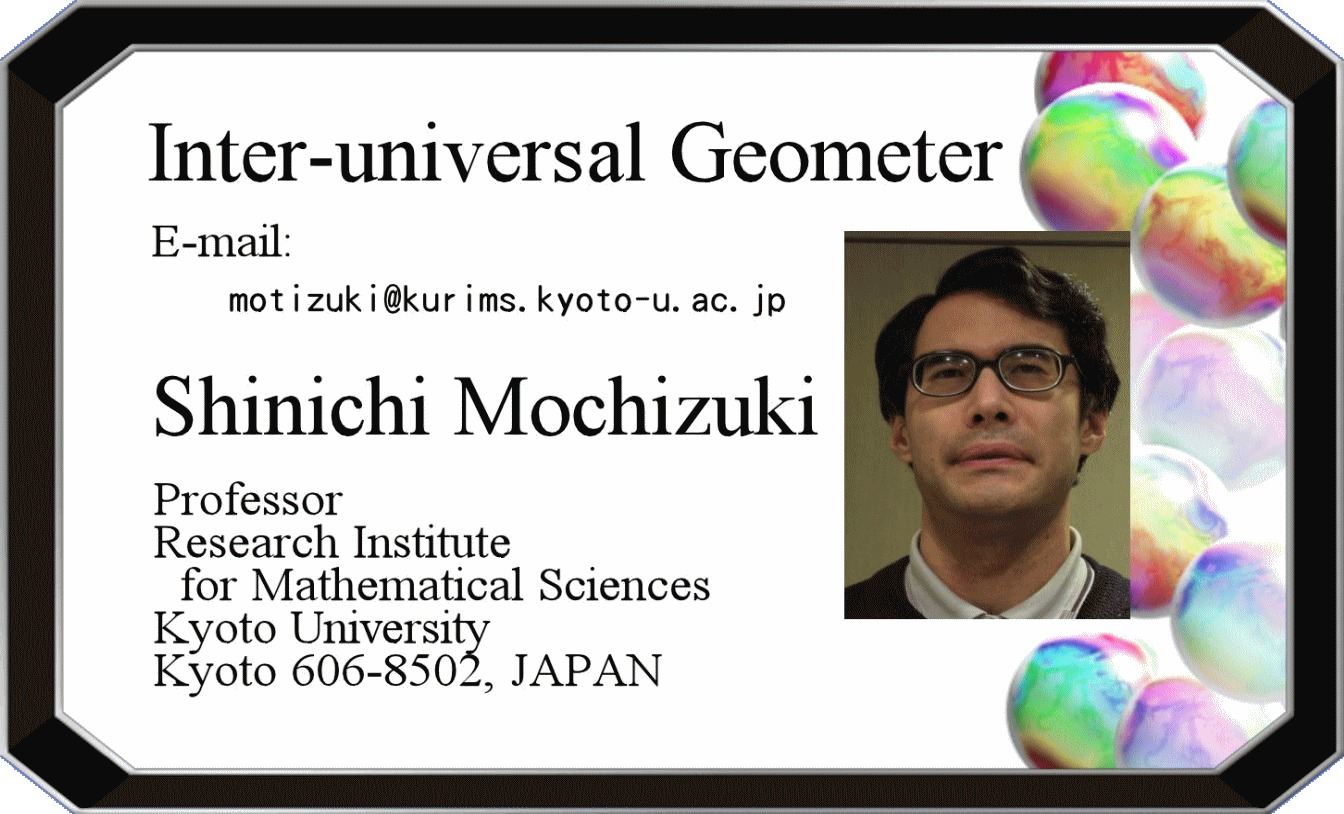
\includegraphics[width=8cm]{mochizuki.jpg}
\end{center}

Here is another result, due to Fabien Pazuki. If $A$ is an abelian variety of
dimension $2$, then it is a Jacobian of some curve, or a product of two elliptic
curves. Namely,

\begin{fact}
  Let $A/K$ be a principally polarized abelian variety of dimension $2$. Then
  \begin{enumerate}
  \item[(1)] either $A \isom \Jac (C)$ for a curve $C$ of genus $2$, polarized
    by $\Theta = C$,

  \item[(2)] or $A \isom E_1\times E_2$ is a product of elliptic curves,
    polarized by $\Theta = E_1\times \{ O \} + \{ O \} \times E_2$.
  \end{enumerate}
\end{fact}

For an archimedian place $v$ on $K$ we have uniformization
$A (\overline{K}_v) \isom \CC^2/\ZZ^2 + \tau_v \, \ZZ^2$, where
$\tau_v = \begin{pmatrix}
  \tau_{1,v} & \tau_{12,v} \\
  \tau_{12,v} & \tau_{2,v}
\end{pmatrix}$.
We call the \term{archimedian trace} of $A$ the quantity
$$\Tr_\infty (A) \dfn \sum_{v \in M_K^\infty} d_v \, \Tr (\Im \tau_v),$$
and the \term{archimedian simplicity} of $A$ is the quantity
$$s_\infty (A) \dfn \prod_{v\in M_K^\infty} |\tau_{12,v}|_v^{d_v}.$$
One has $s_\infty (A) = 0 \iff A\isom E_1\times E_2$.

\begin{theorem}[Pazuki, 2012]
  In case $s_\infty (A) \ne 0$, so that $A \isom \Jac (C)$, for a point
  $P \in A(K)$

  \begin{enumerate}
  \item[(1)] either $[n]\,P = 0$ for $1 \le n \le c_1 (d)$,

  \item[(2)] or $\widehat{h}_{A,2\Theta} (P) \ge c_2 (d) \cdot \left(\Tr_\infty (A) - \frac{5}{3} \, \frac{N_{K/\QQ} (D)}{s_\infty (A)}\right)$,
    where $D\dfn 2^8 \, \disc (F)$, and $F$ is an integral model of the
    hyperelliptic curve $C\colon y^2 = F (x)$.
  \end{enumerate}
\end{theorem}

As a corollary, in case
$\Tr_\infty (A) > \frac{5}{3} \, \frac{N_{K/\QQ} (D)}{s_\infty (A)}$ one obtains
the Lang--Silverman conjecture.

The relation of $\Tr_\infty$ to the Faltings height is the following:
$$h_F (A/K) \le c_3 (d) \cdot \Tr_\infty (A) + c_4 (d)\,\frac{N_{K/\QQ} (D)}{s_\infty (A)},$$
for some $c_3 (d) > 0$, $c_4 (d) > 0$.

For details see \url{http://arxiv.org/abs/0812.2854v2}.

\vspace{1em}

Recall the Lehmer's conjecture for numbers
$h (\alpha) \stackrel{?}{\ge} \frac{1}{[\QQ (\alpha) : \QQ]}\,C$ (where $\alpha$
is not zero and not a root of unity). Similarly we can ask whether for an
abelian variety $A/K$ there is a constant $C (A) > 0$ such that
$\widehat{h}_A (P) \stackrel{?}{\ge} \frac{1}{[\QQ (P) : \QQ]} \, C (A)$ (where
$P$ is not a torsion point). Here we fix $A$ and consider varying $K$, while in
Lang--Silverman we fix $K$ and vary $A$. One result in this direction is the
following.

\begin{theorem}[Ratazzi, 2004]
  Let $E/K$ be an elliptic curve with complex multiplication. There exists a
  constant $c (E/K) > 0$ such that for all
  $P \in E (\overline{K})\setminus E (\overline{K})_\mathrm{tors}$
  $$\widehat{h}_E (P) \ge \frac{c (E/K)}{D} \, \left(\frac{\log\log 5D}{\log 2D}\right)^{13},$$
  where $D \dfn [K^\mathrm{ab} (P) : K^\mathrm{ab}]$.
\end{theorem}

See \url{http://arxiv.org/abs/math/0402225}.

\begin{remark}
  Recall that an elliptic curve $E$ has \term{complex multiplication} if it has
  nontrivial endomorphisms, which means $\End (E) \supsetneq \ZZ$.

  For example, the curve $E\colon y^2 = x^3 - x$ has an extra endomorphism given
  by $i\colon (x,y)\mapsto (-x, i\,y)$.

  Over finite fields an elliptic curve always has extra endomorphisms coming
  from the Frobenius map $x\mapsto x^p$. However, over a number field the
  property of having extra endomorphisms is exceptional.
\end{remark}

In higher dimensions, for abelian varieties with complex multiplication, there
are similar results by Mar\'ia Carrizosa.

\end{document}
